\documentclass[11pt,a4paper]{article}

% ---------- encoding & CJK language ----------
% Compile with xelatex. arXiv supports xelatex via 00README.XXX.
\usepackage{fontspec}
\usepackage{xeCJK}
% Use Fandol fonts (shipped with TeX Live, available on arXiv).
% Reference by filename so xelatex finds them via kpathsea without fontconfig.
\setCJKmainfont{FandolSong-Regular}[
  Extension=.otf,
  BoldFont=FandolSong-Bold]
\setCJKsansfont{FandolHei-Regular}[
  Extension=.otf,
  BoldFont=FandolHei-Bold]
\setCJKmonofont{FandolFang-Regular}[
  Extension=.otf]

% ---------- typography & layout ----------
\usepackage[margin=1in]{geometry}
\usepackage{setspace}
\setstretch{1.25}
\usepackage{parskip}
\widowpenalty=10000
\clubpenalty=10000
\raggedbottom

% ---------- math ----------
\usepackage{amsmath,amssymb,amsthm}
\usepackage{mathtools}

% ---------- unicode glyph coverage for non-CJK prose ----------
\usepackage{newunicodechar}
\newunicodechar{σ}{\ensuremath{\sigma}}
\newunicodechar{Σ}{\ensuremath{\Sigma}}
\newunicodechar{α}{\ensuremath{\alpha}}
\newunicodechar{β}{\ensuremath{\beta}}
\newunicodechar{γ}{\ensuremath{\gamma}}
\newunicodechar{δ}{\ensuremath{\delta}}
\newunicodechar{λ}{\ensuremath{\lambda}}
\newunicodechar{μ}{\ensuremath{\mu}}
\newunicodechar{ϵ}{\ensuremath{\epsilon}}
\newunicodechar{ε}{\ensuremath{\varepsilon}}
\newunicodechar{θ}{\ensuremath{\theta}}
\newunicodechar{π}{\ensuremath{\pi}}
\newunicodechar{ρ}{\ensuremath{\rho}}
\newunicodechar{τ}{\ensuremath{\tau}}
\newunicodechar{φ}{\ensuremath{\varphi}}
\newunicodechar{ψ}{\ensuremath{\psi}}
\newunicodechar{ω}{\ensuremath{\omega}}
\newunicodechar{≈}{\ensuremath{\approx}}
\newunicodechar{≠}{\ensuremath{\neq}}
\newunicodechar{≤}{\ensuremath{\leq}}
\newunicodechar{≥}{\ensuremath{\geq}}
\newunicodechar{±}{\ensuremath{\pm}}
\newunicodechar{×}{\ensuremath{\times}}
\newunicodechar{·}{\ensuremath{\cdot}}
\newunicodechar{→}{\ensuremath{\rightarrow}}
\newunicodechar{←}{\ensuremath{\leftarrow}}
\newunicodechar{↔}{\ensuremath{\leftrightarrow}}
\newunicodechar{∞}{\ensuremath{\infty}}
\newunicodechar{∑}{\ensuremath{\sum}}
\newunicodechar{∏}{\ensuremath{\prod}}
\newunicodechar{∫}{\ensuremath{\int}}
\newunicodechar{∈}{\ensuremath{\in}}
\newunicodechar{∉}{\ensuremath{\notin}}
\newunicodechar{⊂}{\ensuremath{\subset}}
\newunicodechar{⊆}{\ensuremath{\subseteq}}
\newunicodechar{∪}{\ensuremath{\cup}}
\newunicodechar{∩}{\ensuremath{\cap}}
\newunicodechar{∅}{\ensuremath{\emptyset}}
\newunicodechar{↓}{\ensuremath{\downarrow}}
\newunicodechar{↑}{\ensuremath{\uparrow}}
\newunicodechar{—}{---}
\newunicodechar{–}{--}
\newunicodechar{¹}{\textsuperscript{1}}
\newunicodechar{²}{\textsuperscript{2}}
\newunicodechar{³}{\textsuperscript{3}}

% ---------- figures & tables ----------
\usepackage{graphicx}
\graphicspath{{./}}
\usepackage{float}
\usepackage{booktabs}
\usepackage{array}
\usepackage{tabularx}
\usepackage{caption}
\usepackage{tikz}
\usetikzlibrary{arrows.meta,positioning,shapes.geometric,shadows,decorations.pathmorphing}
\captionsetup{font=small,labelformat=empty,justification=centering,
              singlelinecheck=false}

% ---------- hyperlinks & references ----------
\usepackage[hidelinks,breaklinks=true]{hyperref}
\usepackage{xurl}

% ---------- section spacing ----------
\usepackage{titlesec}
\titlespacing*{\section}{0pt}{1.4ex plus .2ex}{0.8ex plus .2ex}
\titlespacing*{\subsection}{0pt}{1.0ex plus .2ex}{0.6ex plus .2ex}
\titlespacing*{\subsubsection}{0pt}{0.8ex plus .2ex}{0.4ex plus .2ex}

% ---------- verbatim blocks ----------
\usepackage{fancyvrb}
\fvset{fontsize=\footnotesize,frame=single,framesep=2mm}

% ---------- centered figures ----------
\makeatletter
\g@addto@macro\@floatboxreset\centering
\makeatother

\title{工业视觉检测中架构感知的解释审计\\
\large 面向模型--解释器--扰动协议的忠实度评估}
\author{}
\date{}
\begin{document}
\maketitle
\thispagestyle{empty}

\textbf{Sibo Jia}\textsuperscript{1} ------ \href{mailto:sibo.jia@ucdconnect.ie}{sibo.jia@ucdconnect.ie} \textbf{Zihang Zhao}\textsuperscript{2} ------ \href{mailto:zihang_zhao@emails.bjut.edu.cn}{zihang\_zhao@emails.bjut.edu.cn}

\textbf{Kunrong Li}\textsuperscript{2} ------ \href{mailto:lkr1213@emails.bjut.edu.cn}{lkr1213@emails.bjut.edu.cn}

\textsuperscript{1} \emph{Dublin College, Beijing University of Technology, Beijing, P.R. China}

\textsuperscript{2} \emph{College of Computer Science, Beijing University of Technology, P.R. China}
\begin{center}
\textbf{摘要}
\end{center}

工业视觉检测系统日益依赖深度分类器，但其热图解释可能在视觉上 看似合理，却未能识别真正驱动模型决策的图像区域。本文将一套 \textbf{架构感知的解释审计协议}操作化于工业视觉检测，其理论基础为 \textbf{原生读出假设}：在指定扰动协议下，解释方法的测量忠实度受其与模型原生决策 机制之间结构距离的约束。在 WM-811K 晶圆图（9 类，172k 样本）上， 采用三种子零填充扰动协议，ViT-Tiny + Attention Rollout 的 Deletion AUC 为 0.211，对比 Swin-Tiny / ResNet18+CBAM / DenseNet121 + Grad-CAM 的 0.432–0.525（|Cohen’s \emph{d}| > 1.1）， 尽管其分类准确率较低。Swin-Tiny 将架构家族与读出结构解耦： 尽管是 Transformer，其空间特征图层级使其与 Grad-CAM 兼容， 表明关键因素是\textbf{读出结构}而非架构家族。模型无关对照（RISE） 将所有家族压缩至 Deletion AUC ≈ 0.1，表明原生方法差距来自解释器通路； 值得注意的是 RISE 优于所有原生方法，因此原生读出是兼容性原则 而非最优性保证。因此，本文不主张存在普适的解释器排序；解释忠实度被视为模型–解释器–扰动三元组的协议条件属性，而非热图方法本身的固有属性。模糊填充敏感性分析表明家族排序在不同扰动基线 下发生反转，强调忠实度排序是（模型、解释器、扰动算子）三元组 的联合属性。在 MVTec AD（预训练模型）上的探索性边界条件研究 确认审计结果依赖于数据集/任务，并识别了需要限定的条件。本协议 提供可操作的指导：解释通路应基于读出结构与模型架构协同设计， 部署的热图应附带定量忠实度指标、模型无关审计基线与明确的扰动协议报告。

\section{引言}

\subsection{研究动机}

深度学习已被部署到许多“仅靠预测结果已不足以交付”的决策场景—— 医疗诊断、自动驾驶、信用评估、工业质量检验等等，都需要一份 可供下游审阅者（医生、工程师、审计员）追问的解释。由此逐渐 形成了一套标准操作流程：先训练尽可能强的分类器，再嫁接一个 事后解释方法，将其热图作为观察模型推理过程的窗口。这种做法 隐含地把解释方法视为\textbf{与所检查分类器相互独立的、中性的测量 工具}。在此假设下，实践者唯一需要考虑的，就是挑选一种计算 廉价、视觉清晰的方法；在 Grad-CAM、积分梯度、LIME 与基于 注意力的方法之间做选择，被简化为便利性问题。本文所汇集的证据 表明，这一假设在系统性且可度量的层面上是错误的。解释方法 相对于它所应用的模型并不中性；其\textbf{忠实度}——即其输出在多大 程度上在指定评估协议下追踪预测相关证据——会因其数学机理与 模型内部决策机制是否匹配而相差两倍以上。

这一问题与从工业 4.0 自动化向工业 5.0 的转型方向一致：工业 5.0 强调以人为本、可持续且具有韧性的生产系统，AI 系统应支持人类 验证而非仅追求预测效率最大化 [21]。制造业与工业信息物理系统中 的 XAI 研究同样强调，可解释性对于提升工业 AI 系统的可信度、 可靠性以及人类对 AI 决策的验证能力至关重要 [22]。在此背景下， 视觉检测中的解释热图应被视为审计工件：它们必须帮助工程师验证 分类器是否依赖有意义的缺陷证据，而非虚假的空间先验。

要严格研究这一主张，需要一个测试平台，其中所比较的模型家族 在架构上差异显著、真值标签信号定义清楚、数据集规模允许多种子 复现的计算开销可接受、并且一份误导性解释的实际代价并不微不 足道。WM-811K 半导体晶圆图数据集 [18] 同时满足这四项条件。 该基准包含 811,457 张晶圆图，其中 172,950 张带有人工标注的 缺陷模式标签，涵盖九个类别，已成为晶圆图缺陷分类的标准测试 平台。当前该基准上的工业 XAI 实践通常完全按上述流程进行—— 训练一个高容量模型、嫁接一个事后解释器、展示热图——忠实度 要么没有论证，要么仅以定性方式主张。因此，WM-811K 在本文中 扮演的是一个具有\textbf{启发性的案例研究}，用于支撑更广泛的 XAI 方法论问题，而非研究本身的终点：下文发展的架构性论断与统计 协议，意在可检验于任何将深度分类器与事后解释器配对的场景， 而不限于特定图像领域。

\subsection{原生读出假设}

本文发展并检验一个机理性假设 —— 即 \textbf{原生读出假设} （native-readout hypothesis）：在文档化的扰动协议下，解释方法的忠实度受其与所解释模型的原生决策机制之间结构距离的约束。在本文中，“原生 读出”指解释方法的数学机理直接读取模型前向决策通路中参与运算的 内部算子（如注意力矩阵），区别于从外部信号（如激活的梯度）重建 重要度的“事后代理”。需注意，“原生”指的是算子对齐，而非因果精确性或与前向计算 完全相同：例如 Attention Rollout 在头间平均并跨层递归相乘，这 并非模型推理时的实际计算，但它读取的是前向传播中路由信息的同一 注意力算子。这里的“结构距离” 通过两个具体指标来操作化。第一个是解释通路究竟是 \emph{直接读出} 模型内部负责信息路由的算子（如 Attention Rollout 直接 读取 Transformer 的注意力矩阵），还是 \emph{从外部通过梯度近似} （如 Grad-CAM 通过卷积激活进行近似）。第二个是解释产出的空间粒度 —— Vision Transformer 的 patch 尺度 vs. 深层卷积块的有效感受野。

在该假设下，可推出五个预测。第一，采用 \emph{原生读出} 的解释方法应产生更低的 Deletion AUC 和更高的 Insertion AUC。 第二，模型家族间的忠实度排序应 \emph{独立于} 其分类性能排序，因为 这两个量度量的是结构上独立的属性。第三，忠实度排序应在不同随机 种子下保持稳定，因为它反映的是架构结构而非学习得到的权重配置。 第四，\emph{模型无关} 的解释器——将模型视为黑盒——应使各家族的忠实度 排序差距大幅压缩，因为它完全绕过了原生读出通路；若差距在模型无关 方法下仍然存在，则效应可归因于架构的表征而非解释器。第五，\emph{层级 Transformer}——使用自注意力但通过多阶段金字塔维持空间特征图—— 应与 Grad-CAM 而非 Attention Rollout 对齐，因为其空间层级提供了 直接的梯度读出路径，尽管底层计算基于注意力；该预测将架构家族 （CNN vs Transformer）与读出结构（空间层级 vs 全局注意力）解耦。 我们将此称为原生读出假设，但在诊断性而非规范性意义上使用该术语。它不是关于解释最优性的形式化理论，而是一个兼容性原则，预测在指定扰动协议下架构特定解释器何时可能具有相对较高的忠实度。它并不意味着原生解释总是比 RISE 等模型无关扰动方法更忠实。因此，本文将 RISE 用作离线审计参考，而非作为与原生解释通路竞争的方法。

本文余下部分在 WM-811K 上检验这五个预测，并在 MVTec AD 上进行 边界条件研究。

\subsection{贡献}

本文贡献有四点。

\textbf{(i) 假设与审计协议。} 本文提出原生读出假设——一个将解释忠实度 与架构–解释器兼容性关联的可证伪结构性主张——并将其操作化为工业 视觉检测的可复用审计协议，为选择模型–解释器对提供可操作的指导。 严格的统计评估设计（每类别拆分、合并 Cohen’s \emph{d}、bootstrap 置信区间、三种子复制）在有限样本预算下加强了推断稳健性。

\textbf{(ii) WM-811K 多家族实证审计。} 对四个模型家族——无注意力 CNN、 注意力增强 CNN、层级 Transformer、全局注意力 Transformer——进行 定量跨架构忠实度审计，填补了晶圆图 XAI 文献停留于定性热图展示 的空白。Swin-Tiny 作为受控证伪测试，将架构家族与读出结构解耦， 证明空间层级而非卷积/注意力之分是 Grad-CAM 兼容性的决定因素。

\textbf{(iii) 对照与消融。} 模型无关对照（RISE）压缩家族间忠实度差距， 表明差距来自解释器通路。针对 ViT 的 2×2 消融设计将 ViT 优势分解为读出直接性 与多层路径深度。模糊填充扰动基线敏感性分析表明家族排序依赖于 协议，强调忠实度排序是（模型、解释器、扰动算子）三元组的联合 属性。

\textbf{(iv) 边界条件分析。} 在 MVTec AD（预训练模型，256×256 RGB）上 的探索性研究用于探查边界条件，而非作为完全匹配的复制；结果表明审计结果依赖于数据集/任务/架构，并识别了假设需要限定 的条件。

\section{相关工作}

\subsection{晶圆图 XAI}

2025–2026 年间对晶圆图分类 XAI 的研究仍是热门方向。Khatun 等 [13] 提出了一个 0.15 M 参数的 CBAM 增强 CNN，在 WM-811K 的平衡 子集上达到 99.88\% 测试准确率，并配合 Grad-CAM、积分梯度 [11] 与遮挡敏感性 [12] 给出预测的解释。Lee 等 [14] 结合 CNN、Grad-CAM、 LIME 与温度缩放，同时报告了准确率、校准性以及双重可视化解释。Park 与 Kim [16] 采用另一条路线，用本身具备可解释性且对标签噪声具备鲁棒 性的模糊推理系统替代 CNN。Lee 等 [15] 则表明 CNN 集成搭配基于 Radon 变换与密度特征可在 WM-811K 上达到 95.09\% 的准确率。上述 工作以及 Pilli [17] 关于人机协同晶圆检测 XAI 的论文，存在 一个共同的结构性局限：每项工作都是将 \emph{某个} 分类器与 \emph{某个} 解释器配对，并且仅以定性方式展示热图，不追问解释器与分类器 在机理上是否相容。

\subsection{更广泛 XAI 文献中的忠实度研究}

在更广泛的可解释性文献中，Jain 与 Wallace [9] 在 NLP 领域记录了 忠实度与合理度之间的差距，表明循环模型中的注意力权重常常对底层 决策并不忠实。Chefer 等 [10] 针对 Vision Transformer，通过将 层级相关性传播（LRP）与注意力梯度结合来填补该差距。Attention Rollout [6] 与 Deletion/Insertion 扰动协议 [7, 8] 提供了本文 使用的度量工具。据作者所知，此前尚未有研究在工业图像基准上 统一检验：解释方法与其模型决策机制之间的结构距离是否能够预测 该方法所能达到的忠实度 —— 本文正是填补该空白的工作。

\subsection{模型无关解释与跨数据集验证}

RISE（随机输入采样解释）[7] 通过随机掩码探测模型并以输出置信度 加权掩码来生成重要性图。由于它将模型视为纯黑盒，可作为区分 架构驱动与解释器驱动忠实度差异的原则性对照。MVTec AD [19] 是 广泛使用的工业异常检测基准，包含 15 个物体类别共 5,354 张图像， 附带像素级缺陷标注。其更高分辨率（700–1024 px）、自然 RGB 图像 及真值掩码使其成为 WM-811K 低分辨率灰度晶圆图的互补测试平台。 DeiT [20] 提供了在 ImageNet 上预训练的数据高效 Vision Transformer 变体，使其能与预训练 CNN 进行公平比较。

\subsection{工业视觉检测中的可信 AI}

从工业 4.0 自动化向工业 5.0 的转型强调以人为本、可持续且具有 韧性的生产系统，AI 系统应支持人类验证而非仅追求预测效率 [21]。 制造业与工业信息物理系统中的 XAI 综述同样强调，可解释性对于 提升可信度、可靠性以及人类对工业 AI 决策的验证能力至关重要 [22]。尽管如此，现有工业检测文献绝大多数仅以定性方式展示热图 ——表明某方法高亮了“正确区域”——而未审计所高亮像素是否真正驱动 模型预测。本文通过将一套定量忠实度审计操作化于任意分类器–解释器 对，填补了这一空白。


\begin{figure}[htbp]
\centering
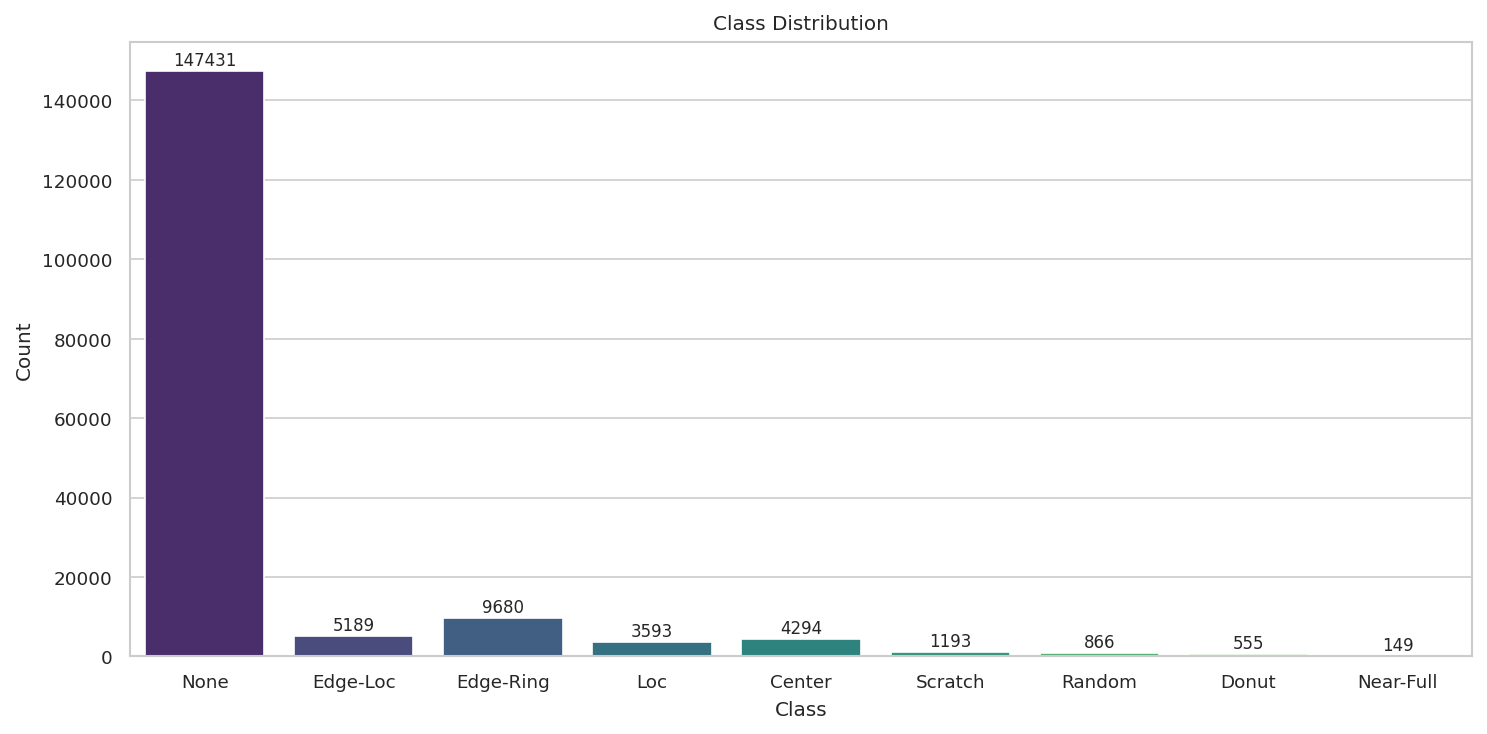
\includegraphics[width=0.55\linewidth]{fig_00.png}
\caption{\textbf{图 1.} WM-811K 有标注样本的类别分布}
\end{figure}

\begin{figure}[htbp]
\centering
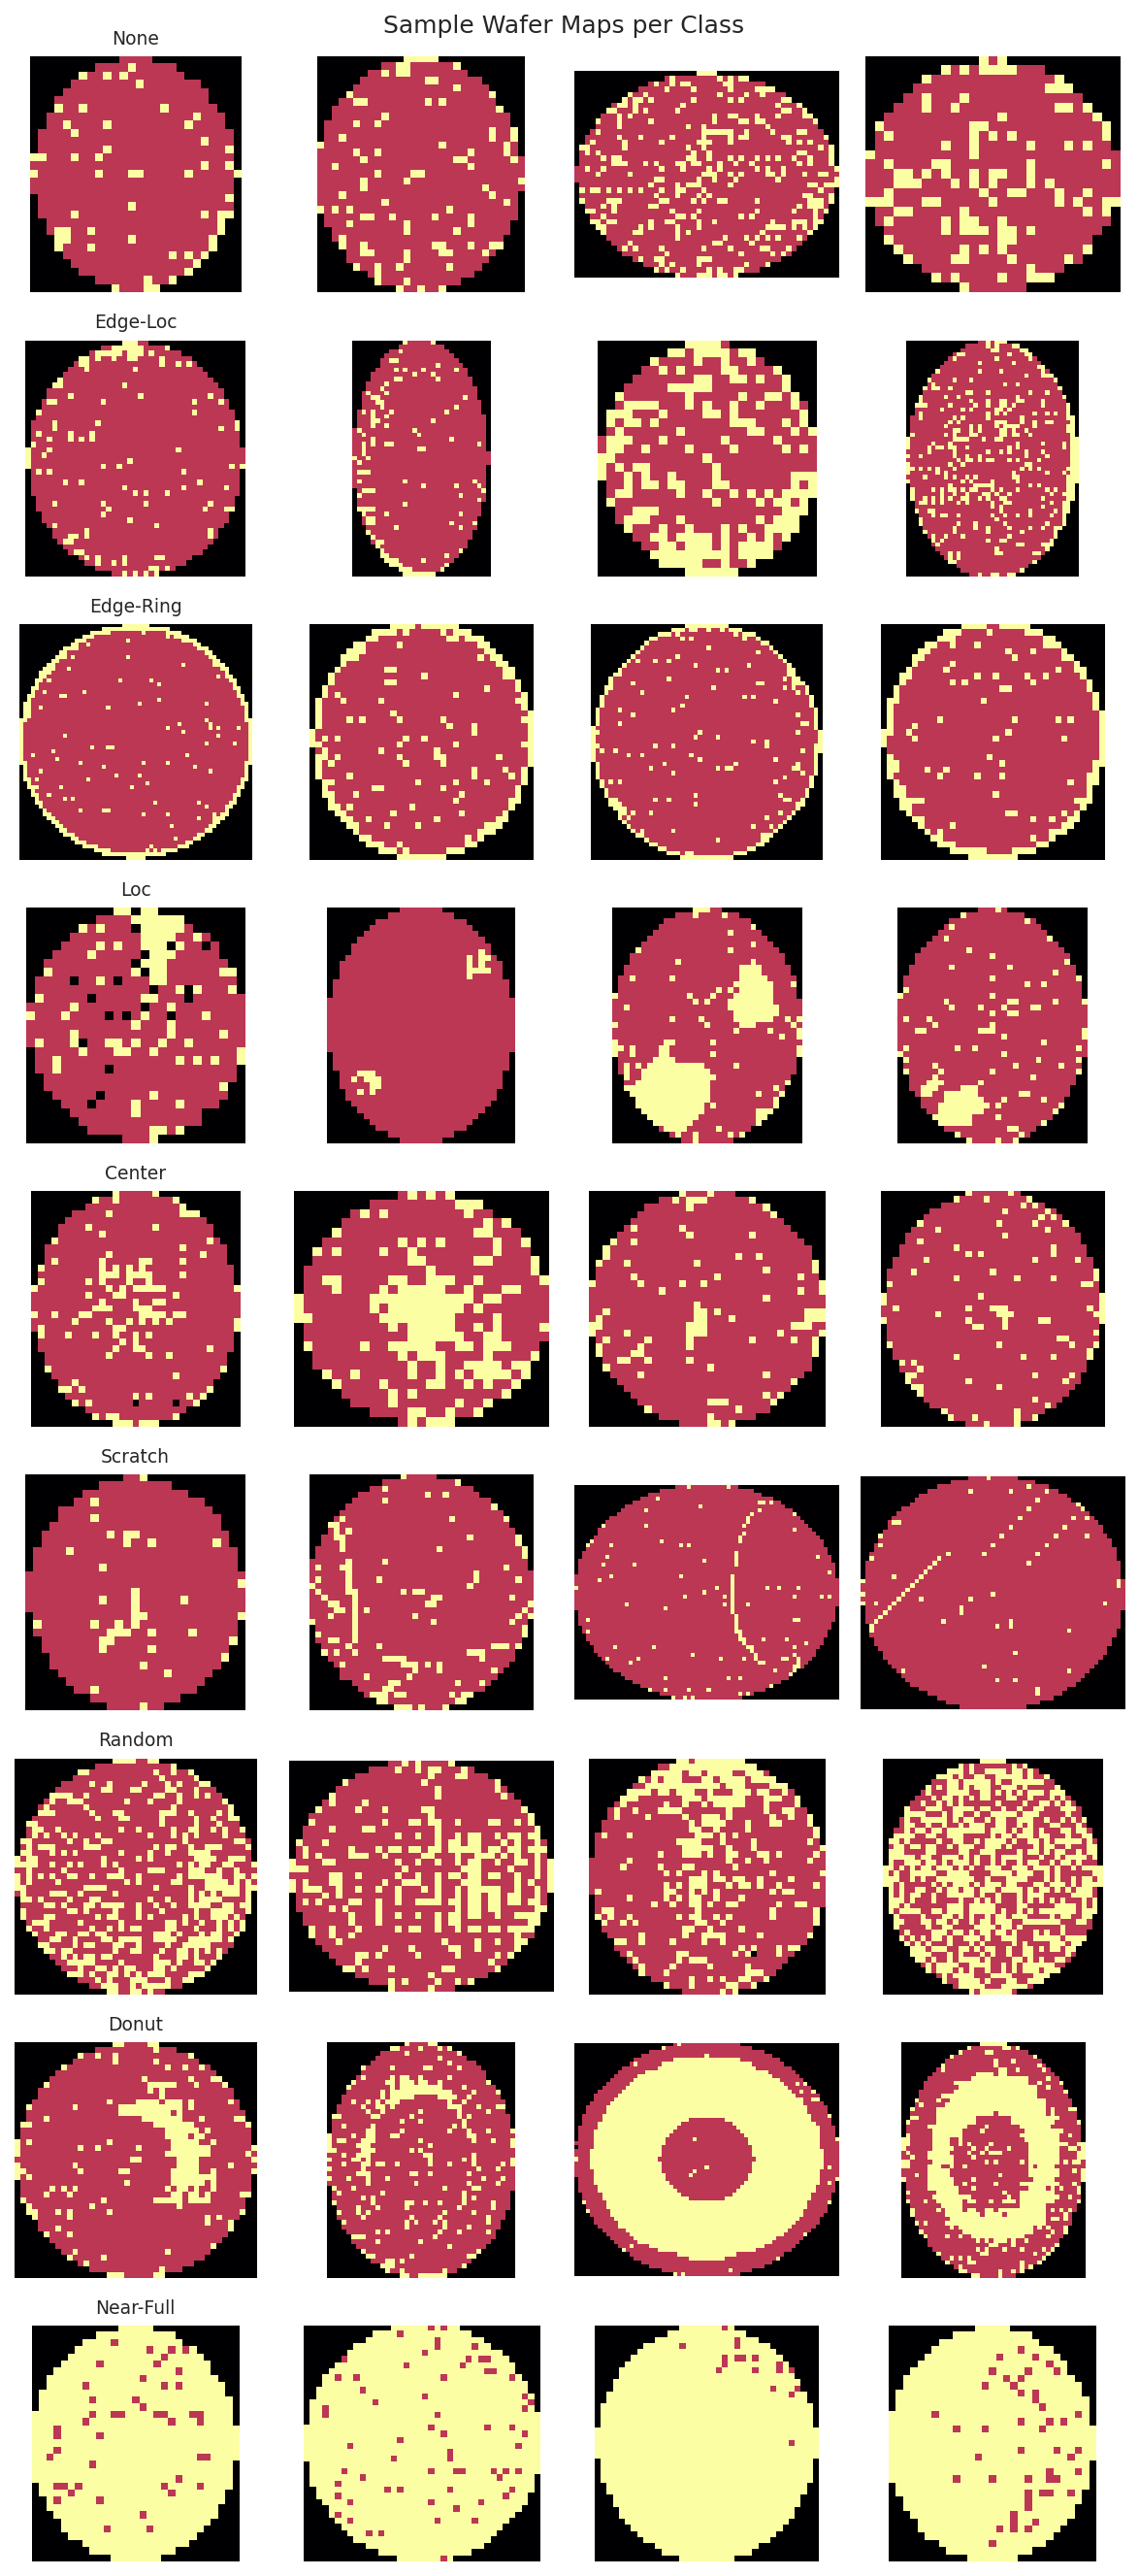
\includegraphics[width=0.55\linewidth]{fig_01.png}
\caption{\textbf{图 2.} 各类别典型晶圆图示例（每类 4 张，64×64）。黑色 = 背景，红色 = 正常芯粒，黄色 = 缺陷芯粒}
\end{figure}

\section{方法}

\subsection{数据集}

WM-811K 基准 [18] 包含 811,457 张晶圆图，其中 172,950 张带有 人工标注的缺陷模式标签，涵盖九个类别（None、Center、Donut、 Edge-Loc、Edge-Ring、Loc、Random、Scratch、Near-Full）。数据集 高度不平衡，约 85\% 的有标注样本属于无缺陷的 “None” 类。图 1–2 分别展示了类别分布与典型晶圆图。由于多数类已占超过五分之四的 有标注样本，原始准确率并不能有效反映模型行为；本研究因此采用 平衡准确率（balanced accuracy）与宏平均 F1 作为主要性能指标， 它们平等对待每一类并对少数类的表现敏感。

数据集按 70 / 15 / 15 比例划分为训练集、验证集与测试集，采用 \textbf{按批次分组划分}（lot-group split）策略。在该方案下，同一生产 批次（lot）的所有晶圆都被限定在同一个子集内，任何批次不会同时 出现在多个子集中。批次由 WM-811K 元数据中的 \texttt{lotName} 字段识别； 缺少有效批次标识的样本（约 0.3\%）被作为单样本组处理。此策略 可以规避信息泄露风险 —— 因为同批次 晶圆之间存在系统性缺陷关联，简单随机划分会使模型利用训练集与 测试集中共享的批次特异模式，从而虚高测试性能。晶圆图通过最近邻 插值被缩放至 64×64，这样可保留离散像素语义（背景/合格/失败）， 而双线性或双三次插值会将这些信息平滑掉。训练样本通过随机旋转、 水平与垂直翻转以及加性高斯噪声（σ=0.05）进行增强。含训练样本 少于 1000 的少数类得到双倍增强概率，该机制在不合成新样本的 前提下部分弥补了类别不平衡。

\subsection{模型架构}

本文比较四个架构上迥异的模型家族，它们分别覆盖了无注意力、 注意力增强、空间层级 Transformer 与全局注意力 Transformer 四类 设计。这一四点设计隔离了注意力机制与空间结构在决策 路径中的角色——从缺失（DenseNet121）、到辅助（ResNet18+CBAM）、到构成性但局部/层级化（Swin-Tiny）、再到构成性且全局化（ViT-Tiny）——从而可以受控地检验解释方法与原生决策 机制之间的结构距离如何影响忠实度。

\subsubsection{ResNet18 + CBAM}

ResNet-18 [1] 提供了一个坚实的卷积基线，其核心构件实现残差映射：

\begin{equation}
\mathbf{y} = \mathcal{F}(\mathbf{x}, \{W_i\}) + \mathbf{x}
\tag{1}
\end{equation}

其中 $\mathcal{F}$ 由若干卷积、批归一化和 ReLU 层堆叠组成。 卷积块注意力模块（CBAM [2]）被附加在四个残差阶段之后。CBAM 分 两步顺序细化输入的特征图。通道注意力分支计算：

\begin{equation}
M_c(\mathbf{F}) = \sigma\!\left(\text{MLP}(\text{AvgPool}(\mathbf{F})) + \text{MLP}(\text{MaxPool}(\mathbf{F}))\right)
\tag{2}
\end{equation}

随后是空间注意力分支：

\begin{equation}
M_s(\mathbf{F}') = \sigma\!\left(f^{7{\times}7}\!\left([\text{AvgPool}(\mathbf{F}');\, \text{MaxPool}(\mathbf{F}')]\right)\right)
\tag{3}
\end{equation}

得到 $\mathbf{F}'' = M_s(\mathbf{F}') \odot \mathbf{F}'$， 其中 $\mathbf{F}' = M_c(\mathbf{F}) \odot \mathbf{F}$。由于两个 门控信号都是显式的架构组件，该家族体现了“按设计注意” （attention-by-design）的特征选择方式。

\subsubsection{DenseNet121}

DenseNet-121 [3] 使用稠密的层间连接而非显式注意力机制。在 dense block 内部，第 $\ell$ 层接收此前所有层特征图的拼接：

\begin{equation}
\mathbf{x}_\ell = H_\ell\!\left([\mathbf{x}_0,\, \ldots,\, \mathbf{x}_{\ell-1}]\right)
\tag{4}
\end{equation}

其中 $H_\ell$ 是批归一化、ReLU 和 3×3 卷积的组合。该架构不包含 任何显式注意力机制，因此作为一个干净的黑盒卷积基线：任何可解释 信号都必须通过事后梯度或扰动来恢复。

\subsubsection{ViT-Tiny}

Vision Transformer [4] 将输入处理为一串不重叠的图像块（patch）， 每个 patch 经线性映射至固定维度的嵌入，并与一个可学习的 [CLS] token 拼接：

\begin{equation}
\mathbf{z}_0 = [\mathbf{x}_{\text{cls}};\; \mathbf{x}_1^p E;\; \ldots;\; \mathbf{x}_N^p E] + \mathbf{E}_{\text{pos}}, \quad N = HW / P^2
\tag{5}
\end{equation}

每一个编码器层应用多头自注意力：

\begin{equation}
\text{Attn}(Q, K, V) = \text{softmax}\!\left(\frac{QK^\top}{\sqrt{d_k}}\right)V
\tag{6}
\end{equation}

随后接前馈网络和残差连接。本文采用的配置：patch 尺寸 $P{=}4$ （对 64×64 输入得到 $N{=}256$ 个 token），嵌入维度 192，深度 12， 注意力头数 3。ViT-Tiny 不具备任何卷积归纳偏置，所有 patch 间 空间关系都由学习得到的注意力权重涌现出来，因此是该对比中典型 的“注意力优先”（attention-first）架构。

\subsubsection{Swin-Tiny}

Swin Transformer [23] 通过将自注意力与层级空间结构相结合，架起了 CNN 与 ViT 之间的桥梁。与 ViT 从第一层即对所有 patch 施加全局 注意力不同，Swin 将注意力限制在局部窗口内，并通过移位窗口分区 引入跨窗口连接：

\begin{equation}
\text{W-MSA}(\mathbf{z}^{\ell}) = \text{Concat}\left(\text{Attn}(Q_w, K_w, V_w)\right)_{w=1}^{M^2}
\tag{7}
\end{equation}

其中每个窗口 $w$ 包含 $M{\times}M$ 个 token（WM-811K 64×64 输入 时 $M{=}4$，MVTec 256×256 输入时 $M{=}7$）。该架构包含四个阶段， 通过 patch 合并实现逐步 2× 空间下采样，在每个阶段产生空间特征图——结构上类似于 ResNet 的 layer1–4 或 DenseNet 的 denseblock1–4——尽管底层计算完全基于 注意力。

该架构选择对可解释性有直接影响：Swin 的最终阶段产生空间特征图 （而非全局 token 序列），使其成为 Grad-CAM 的有效目标层。因此 该模型在实验设计中占据独特位置：它是 Transformer（自注意力是 唯一计算原语），但其读出结构是空间的（具有逐步下采样的层级特征 图）。若 Grad-CAM 兼容性取决于架构家族，Swin 应表现得像 ViT； 若取决于读出结构，Swin 应表现得像 CNN。这一受控对比是预测 5 （§1.2）的基础。

\begin{table}[htbp]
\centering
\small
\caption{\textbf{表 1.} 模型家族概览}
\begin{tabular}{llrr}
\toprule
家族 & 描述 & 参数量 & 训练轮数 (主种子) \\
\midrule
ResNet18+CBAM & CNN + 设计的注意力模块 & 11,219,793 & 31 \\
DenseNet121 & 纯 CNN & 6,956,809 & 28 \\
ViT-Tiny & 纯 Transformer & 5,393,289 & 82 \\
Swin-Tiny & Hierarchical Transformer & 27,504,723 & 90 \\
\bottomrule
\end{tabular}
\end{table}

\subsection{可解释性方法}

本节为每个家族配对最自然的解释方法，并在统一的忠实度协议 （§3.4）下对三种方法进行评估。配对方式是刻意选择的：Grad-CAM 读取 CNN 用于空间编码的最终卷积特征图，而 Attention Rollout 读取构成 Transformer 原生信息路由机制的注意力矩阵。这一设计 旨在最大化每个家族的忠实度上限，并降低观察到的差异仅由方法 选择的次优性驱动的风险。

\subsubsection{Grad-CAM（面向 CNN 与 Swin）}

Grad-CAM [5] 通过流入目标卷积层的梯度生成类别判别热图。对于 目标类 $c$ 与所选层的特征图 $A^k$：

\begin{equation}
\alpha_k^c = \frac{1}{Z} \sum_i \sum_j \frac{\partial y^c}{\partial A^k_{ij}}
\tag{8}
\end{equation}

\begin{equation}
L_{\text{Grad-CAM}}^c = \text{ReLU}\!\left(\sum_k \alpha_k^c A^k\right)
\tag{9}
\end{equation}

ReLU 仅保留对类别 $c$ 有正向影响的特征；结果被上采样至输入 分辨率并通过最大最小归一化缩放到 $[0, 1]$。在原生读出框架中， Grad-CAM 占据一个特定位置：它是 CNN 决策机制的 \textbf{基于梯度的代理}， 而非其直接读出。CNN 的原生决策算子是学习到的卷积核及其所产生的 空间特征图；然而，这些特征图无法单独作为类别特异性解释——数百张 特征图同时响应不同模式，且没有内建机制指示哪些空间位置驱动了 特定类别的决策。Grad-CAM 通过将目标 logit 的梯度沿这些卷积核 反向传播并对激活加权来弥合这一缺口，但这种重建本质上是间接的。 目标层的选择部分控制了结构距离：ResNet18+CBAM 使用 \texttt{cbam4} （分类器消费的注意力后特征图），DenseNet121 使用 \texttt{features.denseblock4}（全局池化前的最后一个稠密块）。两种选择 都在“不存在显式路由信号可读”的约束下尽量减小结构距离。 对 Swin-Tiny，目标层为最终 Transformer 阶段 \texttt{layers[-1]}。 该阶段输出空间特征图（2×2），因此可作为 Grad-CAM 的目标层； 尽管其底层计算完全基于窗口自注意力，但其最终读出结构与 CNN 的最后空间特征块在功能上相似。

\subsubsection{Attention Rollout（面向 ViT）}

Attention Rollout [6] 累积所有 Transformer 层的注意力来估计 每个输入 patch 对最终 [CLS] token 的贡献程度。在第 $\ell$ 层， 原始注意力矩阵 $A^{(\ell)} \in \mathbb{R}^{N \times N}$ 先 在头之间平均，再与单位矩阵相加以纳入残差连接的贡献：

\begin{equation}
\hat{A}^{(\ell)} = 0.5 \cdot \bar{A}^{(\ell)} + 0.5 \cdot I
\tag{10}
\end{equation}

随后 Rollout 递归地相乘：

\begin{equation}
R^{(\ell)} = \hat{A}^{(\ell)} \cdot R^{(\ell-1)}, \quad R^{(0)} = I
\tag{11}
\end{equation}

最终热图是 $R^{(L)}$ 的 [CLS] 行，经重排到空间网格后归一化。 在原生读出框架中，Attention Rollout 占据对立位置：它是 Transformer 信息路由结构的 \textbf{更近前向通路读出}（相比基于梯度的 事后代理）。Transformer 的注意力矩阵是其原生信息路由通路的 组成部分，控制信息如何从 patch token 流向分类器所消费的 [CLS] token。Rollout 通过 (式 10) 的残差通路 以及 (式 11) 的 12 层递归乘积累积这些矩阵，整个过程不涉及梯度： 解释是从产生预测的同一前向过程中计算出来的，所报告的量即 决策本身的一阶属性。与 Grad-CAM 不同，Rollout 并非显式的类别 判别方法——它估计的是 token 对 [CLS] 通路的信息贡献，而不直接 针对某个类别 logit。在本文中，Rollout 仍以预测类别概率作为 Deletion/Insertion 的评估目标，因此忠实度问题是：该 [CLS] 信息 路由图是否识别了模型用于自身预测的像素。Chefer 等 [10] 更近期的类别特定方法将 LRP 与注意力梯度结合；本文仍保留 Rollout，\emph{恰恰因为} 它是 Transformer 路由矩阵的最小距离读出，因此是检验原生读出假设的最干净工具。

需要注意的是，Attention Rollout 并未应用于 Swin-Tiny。Swin 不包含全局 [CLS] token，其分类头作用于最终阶段输出的空间平均特征；同时，其窗口注意力矩阵并不形成全局 token-to-token 路由路径。这种架构不兼容性本身说明 Swin 的读出结构更接近空间层级模型，而非全局注意力 ViT，因此本文对该家族采用 Grad-CAM。

\subsubsection{RISE（模型无关对照）}

RISE（Randomized Input Sampling for Explanation）[7] 通过随机掩码 输入探测模型来生成重要性图。采样 $N$ 个分辨率为 $s{\\times}s$ （默认 $s{=}8$）的二值掩码，经双线性插值上采样至输入尺寸后逐 元素乘以输入图像。记录每个掩码下模型对目标类别的输出置信度， 最终显著性图为所有掩码的置信度加权平均：

\begin{equation}
S(x) = \frac{1}{N} \sum_{i=1}^{N} f_c(x \odot M_i) \cdot M_i
\tag{12}
\end{equation}

其中 $f_c$ 为模型对类别 $c$ 的 softmax 概率，$M_i$ 为第 $i$ 个 上采样掩码。由于 RISE 将模型视为纯黑盒——不使用梯度、内部激活 或架构特定钩子——它为解耦架构驱动与解释器驱动的忠实度差异提供 了原则性对照。若原生方法优于 RISE，则优势可归因于解释器与模型 的结构对齐；若 RISE 匹配或超越原生方法，则原生通路未提供额外 忠实度收益。本研究中，WM-811K 和 MVTec AD 评估均使用 $N{=}4000$ 个掩码、分辨率 $8{\\times}8$。

\begin{table}[htbp]
\centering
\small
\caption{\textbf{表 2.} 可解释性方法分配}
\begin{tabular}{llll}
\toprule
家族 & 方法 & 目标层 & 读出类型 \\
\midrule
ResNet18+CBAM & Grad-CAM (式 8-9) & cbam4 & 事后代理（梯度） \\
DenseNet121 & Grad-CAM (式 8-9) & features.denseblock4 & 事后代理（梯度） \\
Swin-Tiny & Grad-CAM (式 8-9) & layers[-1]（最终阶段） & 事后代理（梯度） \\
ViT-Tiny & Attention Rollout (式 10-11) & 全部 12 个编码器层 & 原生读出（前向） \\
所有家族 & RISE (式 12) & 黑盒（N=4000 掩码） & 模型无关 \\
\bottomrule
\end{tabular}
\end{table}

由于每种架构配对其最自然的解释器，主要比较评估的是模型–解释器 对而非单独的架构；将架构效应与解释器效应解耦需要 §S9 和 §S10 中报告的消融实验（在 §5.1 和局限性部分（§5.7）中讨论），将差距分解为 ≈42\% 读出直接性和 ≈52\% 路径深度。


\subsection{训练与评估协议}

\subsubsection{训练}

四个家族共享统一的优化框架。根据各家族配置，优化器使用 Adam 或 AdamW，学习率调度为余弦退火或 plateau 降学习率。早停对 CNN 家族基于验证集平衡准确率触发，对 ViT-Tiny 基于验证集 macro-F1 触发（详见补充表 S1），以更好反映不平衡的目标。由于 ViT-Tiny 缺乏卷积归纳偏置而收敛较慢，其最大训练轮数设置更大； 比较均使用最佳验证检查点而非最终轮次。每次训练运行 都会将完整配置写入所在目录的 \texttt{config.yaml}，使得任何实验都能从 其保存的产物中精确重建。每个家族的完整超参详见补充表 S1。

\subsubsection{随机种子与方差估计}

为估计不同运行间的方差而不是仅报告单次点估计，每个家族在三个 随机种子下训练，共十二个 WM-811K 运行。ResNet18+CBAM、DenseNet121 和 ViT-Tiny 使用种子 42、123、456；Swin-Tiny 使用种子 7、123、456 （种子 42 对该家族产生退化初始化；详见补充材料 §S13）。所有报告 的指标均按这些种子取均值 ± 标准差。逐种子分类结果见补充表 S3。


\subsubsection{忠实度指标}

解释质量通过三个互补指标评估，三者对所有家族使用完全相同的 计算流程。

\textbf{Deletion AUC} [7] 按热图排名由高到低逐步将像素置零，并跟踪 预测类别的概率：

\begin{equation}
\text{Del-AUC} = \int_0^1 P\bigl(c \mid x_{\setminus \text{top-}f}\bigr)\, df
\tag{13}
\end{equation}

忠实的解释会优先排序与决策相关的像素，导致概率迅速下降，进而 得到 \textbf{较小} 的 AUC。

\textbf{Insertion AUC} [7] 从全零图像出发，按排名逐步插入得分最高的像素：

\begin{equation}
\text{Ins-AUC} = \int_0^1 P\bigl(c \mid x_{\text{top-}f}\bigr)\, df
\tag{14}
\end{equation}

忠实的解释能以少量像素恢复置信度，进而得到 \textbf{较大} 的 AUC。

\textbf{Stability} [8] 度量热图在语义保持扰动下的一致性。对于 $K{=}5$ 种增强（旋转 ±15°、平移 ±3 px、高斯噪声 σ=0.02）：

\begin{equation}
\text{Stability} = \frac{1}{K}\sum_{k=1}^K \frac{\langle h(x),\, h(x_k')\rangle}{\|h(x)\| \cdot \|h(x_k')\|}
\tag{15}
\end{equation}

该指标只在晶圆区域（像素值 > 0）上计算。所有扰动曲线均针对 模型预测类别的概率计算，因此该评估衡量的是解释对模型自身决策 路径的忠实度，而不是相对于真实标签的正确性。这些扰动指标在 本文中被视为给定零填充协议下模型–解释器忠实度的代理度量， 而非像素级真实因果解释。模糊填充敏感性检验（§4.6）测试了家族 排序对该基线选择的稳健性。

除非另有说明，本文中“忠实度”均指协议条件下的扰动忠实度：即热图排序在多大程度上识别出那些在指定扰动算子下移除或插入后会改变模型预测类别概率的像素。因此，它是模型–解释器对齐的代理度量，而非因果解释真值的直接度量。

\subsubsection{样本量与统计分析}

上述指标在每个种子上基于 200 个均衡分层采样的测试样本计算 （每类 22 个 × 9 类 = 198 个有效样本，因整数取整所致；每家族 跨 3 个种子合计 594 个样本）。Deletion 与 Insertion AUC 在 20 个 扰动步上计算，覆盖从 0 到 100\% 排序像素的完整范围。对于补充的 top-k 置信度下降分析（§S12），默认阈值为 10\% 的像素（4,096 中 的 410 个），足够精细以区分局部缺陷，同时又足够粗以避免对单 像素噪声敏感。每样本 5 次增强是估计余弦相似度方差的最小数量， 同时能将单 GPU 上的总评估时间控制在可承受范围内。完整参数设置 见补充表 S2。

除了现有晶圆 XAI 文献常用的“均值 ± 标准差”汇总之外，本文还采用 三项互补的统计分析：(i) 对 Deletion AUC 进行按类别拆分，以核实 结论不是由某个有利的类别子集驱动；(ii) 计算合并 Cohen's \emph{d} [effect size] 以量化家族差异的标准化幅度；(iii) 使用非参数 bootstrap（2,000 次重采样）给出每家族 Deletion AUC 均值的 95\% 置信区间。

\subsection{模型无关对照：RISE}

为检验第四个预测（§1.2）——模型无关解释器应大幅压缩各家族之间 的忠实度排序差距——本文对 WM-811K 上的四个家族统一施加 RISE [7] （详见 §3.3.3）。使用相同的 $N{=}4000$ 个掩码、分辨率 $8{\times}8$，所得热图使用与原生方法相同的 Deletion/Insertion 协议（§3.4.3）进行评估，以实现直接比较。RISE 超参数 （$N{=}4000$，掩码分辨率 $8{\times}8$，概率 $p{=}0.5$）在所有 家族间保持一致。

\subsection{边界条件数据集：MVTec AD}

为探查 WM-811K 之外的边界条件，本文将相同审计流程应用于 MVTec AD [19]——一个包含 15 个物体类别（如地毯、皮革、金属螺母、 晶体管）共 5,354 张图像并附带像素级缺陷掩码的工业异常检测基准。该研究并非完全匹配的复制：它使用 RGB 自然图像、ImageNet 预训练骨干、二分类任务以及单一评估种子。

\textbf{任务设定。} 所有类别汇总为二分类任务（正常 vs. 缺陷： 4,096 / 1,258 样本）。70/15/15 分层随机划分产生 3,748 训练、 803 验证和 803 测试样本。

\textbf{预处理。} 图像缩放至 256×256 并按 ImageNet 统计量归一化。 数据增强与 WM-811K 一致（旋转、翻转、高斯噪声）。

\textbf{模型。} 使用相同的四个架构家族，均采用 ImageNet 预训练骨干：ResNet18+CBAM (torchvision)、DenseNet121 (torchvision)、ViT-Tiny (DeiT-Tiny [20], timm) 和 Swin-Tiny [23] (timm)。预训练是必要的，因为 MVTec AD 的自然 RGB 图像和小样本量使 ViT 无法有效地从头训练（经验证实： 从头训练的 ViT 仅达到 55\% 平衡准确率）。所有模型使用 AdamW、 余弦学习率调度和早停（patience 15）进行微调。单一种子（42）用于边界条件研究。

\textbf{可解释性评估。} 对 200 个缺陷测试样本（seed 42）评估原生方法 （CNN 的 Grad-CAM、ViT 的 Attention Rollout）和 RISE。除 Deletion/Insertion AUC 外，像素级真值掩码还可计算热图与真实 缺陷区域之间的 IoU（交并比）。

\textbf{RISE 掩码分辨率消融。} 由于 MVTec 图像比 WM-811K 大 4 倍 （256 vs 64 px），默认 $8{\times}8$ 掩码网格产生 32 px 的单元格 ——对细粒度缺陷可能过于粗糙。对掩码分辨率 $\{8, 16, 32\}$ 的 消融检验 RISE 在该数据集上的性能是否受分辨率限制。

所有代码、配置和评估脚本均公开可用（补充 §S14）。


\section{结果}

\subsection{分类性能}

表 3 给出四个家族在三个随机种子上平均后的分类性能。

\begin{table}[htbp]
\centering
\small
\caption{\textbf{表 3.} 分类性能（在 3 个种子上计算的均值 ± 标准差）}
\resizebox{\linewidth}{!}{%
\begin{tabular}{lrrrrr}
\toprule
家族 & 准确率 & 平衡准确率 & 宏 F1 & 加权 F1 & MCC \\
\midrule
ResNet18+CBAM & 0.957 ± 0.004 & 0.901 ± 0.001 & 0.849 ± 0.005 & 0.960 ± 0.003 & 0.858 ± 0.011 \\
DenseNet121 & 0.962 ± 0.004 & 0.901 ± 0.007 & 0.853 ± 0.011 & 0.964 ± 0.003 & 0.872 ± 0.011 \\
ViT-Tiny & 0.928 ± 0.007 & 0.799 ± 0.014 & 0.747 ± 0.008 & 0.935 ± 0.005 & 0.774 ± 0.019 \\
Swin-Tiny & 0.953 ± 0.002 & 0.822 ± 0.015 & 0.792 ± 0.004 & 0.957 ± 0.002 & 0.838 ± 0.002 \\
\bottomrule
\end{tabular}
}
\end{table}

ViT-Tiny 在宏 F1 上落后两个 CNN 家族约 10 个百分点。这一差距 符合预期也有充分文献佐证 [4, 23]：Vision Transformer 缺乏卷积的 归纳偏置（平移等变性、局部连接性），在小规模、低分辨率数据集上 CNN 因此拥有较强的空间先验。在缺乏大规模预训练（对 64×64 单通道 晶圆图而言并不现实）的情况下，ViT 必须从零学习全部空间关系， 需要大幅更多的训练轮数（67–94 vs. 28–36），且最终仍收敛到更弱 的最优解。关键在于，这一分类劣势并不会使可解释性比较失效，但它要求将忠实度结果与预测性能分开解读。因此，后文的共同正确子集分析与 RISE 对照对于降低“忠实度差距只是分类质量副产品”的风险至关重要。

每类 F1 的雷达图见图 3，每个家族的训练与验证损失曲线见 补充图 S1。


\begin{figure}[htbp]
\centering
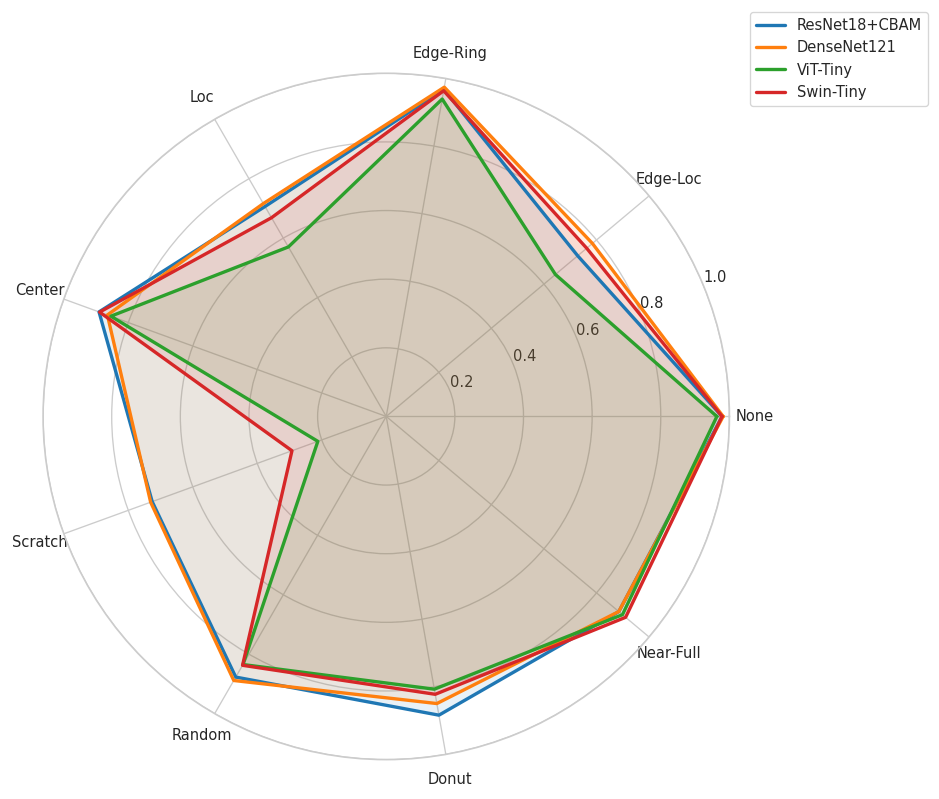
\includegraphics[width=0.55\linewidth]{fig_02.png}
\caption{\textbf{图 3.} 各类别 F1 雷达图（3 个种子的均值）}
\end{figure}

\subsection{定性可解释性分析}

在报告定量忠实度指标（§4.3）之前，本小节先对热图进行定性考察。 在架构迥异的模型家族之间比较可解释性方法在方法论上颇为微妙： CNN 上的 Grad-CAM 与 Transformer 上的 Attention Rollout 来自 数学上不同的对象 —— 前者是梯度加权的激活，后者是注意力矩阵的 累积乘积 —— 因此二者热图的视觉相似度并不直接可比。然而在原生 读出假设下，这种“不可共度”正是本文要研究的对象。评估因此比较 的是每种方法的 \emph{输出行为} —— 移除 top 像素时置信度下降多少、 逐步加回时回升多少、扰动下排名的稳定性如何 —— 而不是热图的 表面外观。本文不试图恢复对任何具体预测因果层面“真正的”解释， 因为 WM-811K 并未提供像素级真值。本文支持的主张形式为“在 Deletion 扰动下，家族 X 的解释比家族 Y 更忠实地跟踪其预测”—— 这类主张是可度量、可复现且与假设相关的。

对于每个类别，选取 ResNet18+CBAM 作为参考，取置信度最高且 分类正确的测试样本，结果见图 5：两个 CNN 家族覆盖 Grad-CAM 叠加层，ViT-Tiny 覆盖 Attention Rollout。在查看完整面板之前， 图 4a–4c 先展示 \textbf{Center} 类的放大对比——该类别是三种方法 差异最为显著的模式。


\begin{figure}[htbp]
\centering
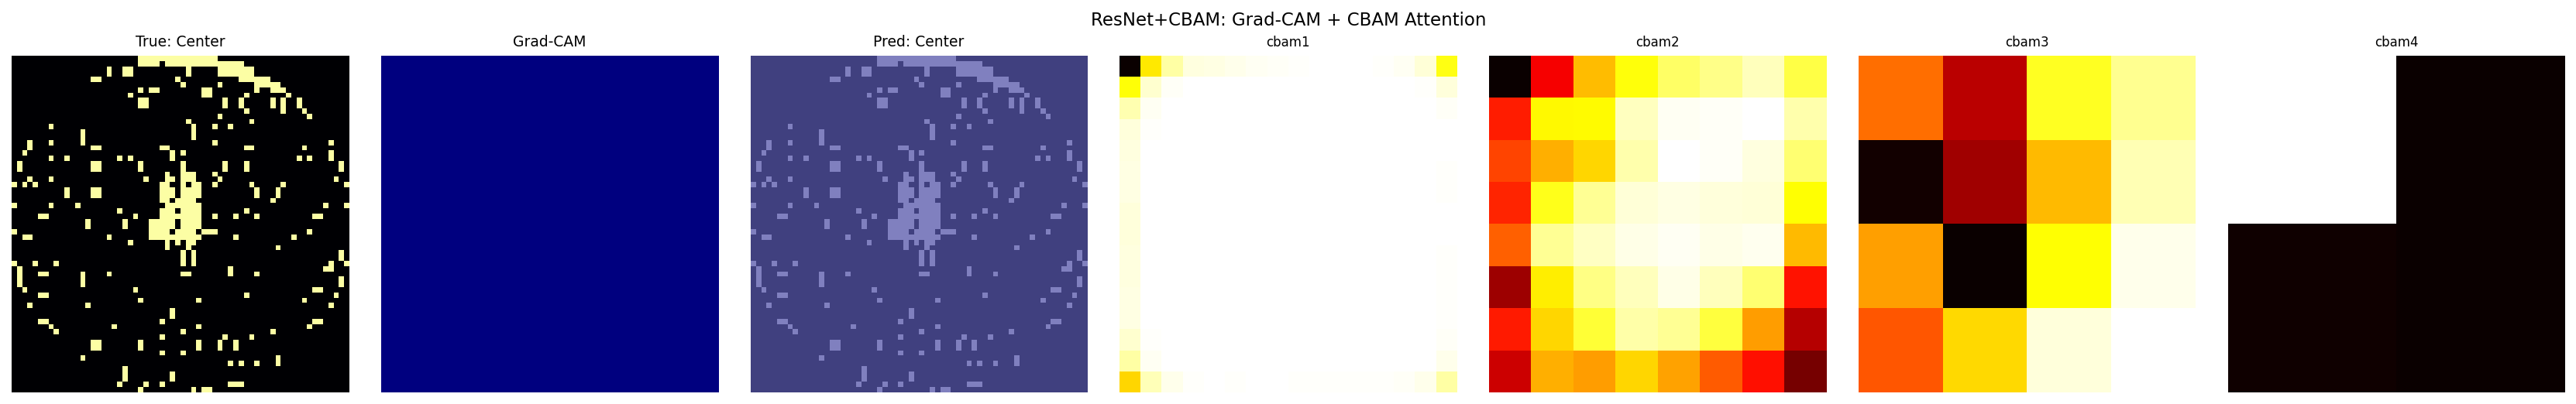
\includegraphics[width=0.98\linewidth]{fig_03.png}
\caption{\textbf{图 4a.} ResNet18+CBAM —— Center 类解释。从左至右：原始晶圆、Grad-CAM 热图、预测叠加图、以及 CBAM 各层（1–4）的空间注意力图。Grad-CAM 几乎均匀暗蓝（退化），未能提供任何缺陷空间定位。CBAM 注意力图（cbam2–cbam3）呈现粗粒度的象限级模式，体现了事后梯度信号在该样本上未能提供有效的缺陷空间定位}
\end{figure}

\begin{figure}[htbp]
\centering
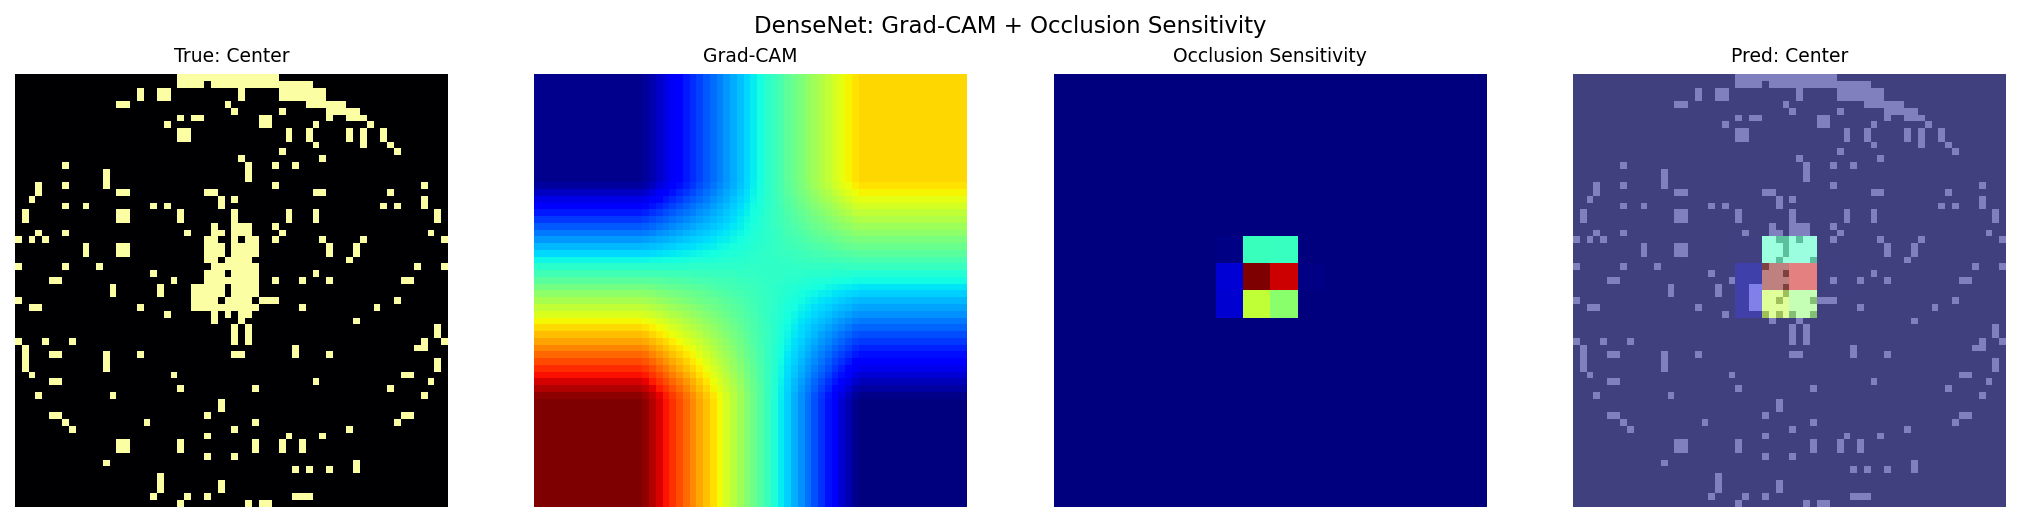
\includegraphics[width=0.98\linewidth]{fig_04.png}
\caption{\textbf{图 4b.} DenseNet121 —— Center 类解释。从左至右：原始晶圆、Grad-CAM 热图、遮挡敏感性图、预测叠加图。Grad-CAM 将热区置于左下角——远离中心缺陷簇——表明梯度代理在该样本上未能恢复缺陷位置。遮挡敏感性图（模型无关的参考方法）则正确定位了中心区域，凸显了梯度路径报告与模型实际敏感区域之间的差距}
\end{figure}

\begin{figure}[htbp]
\centering
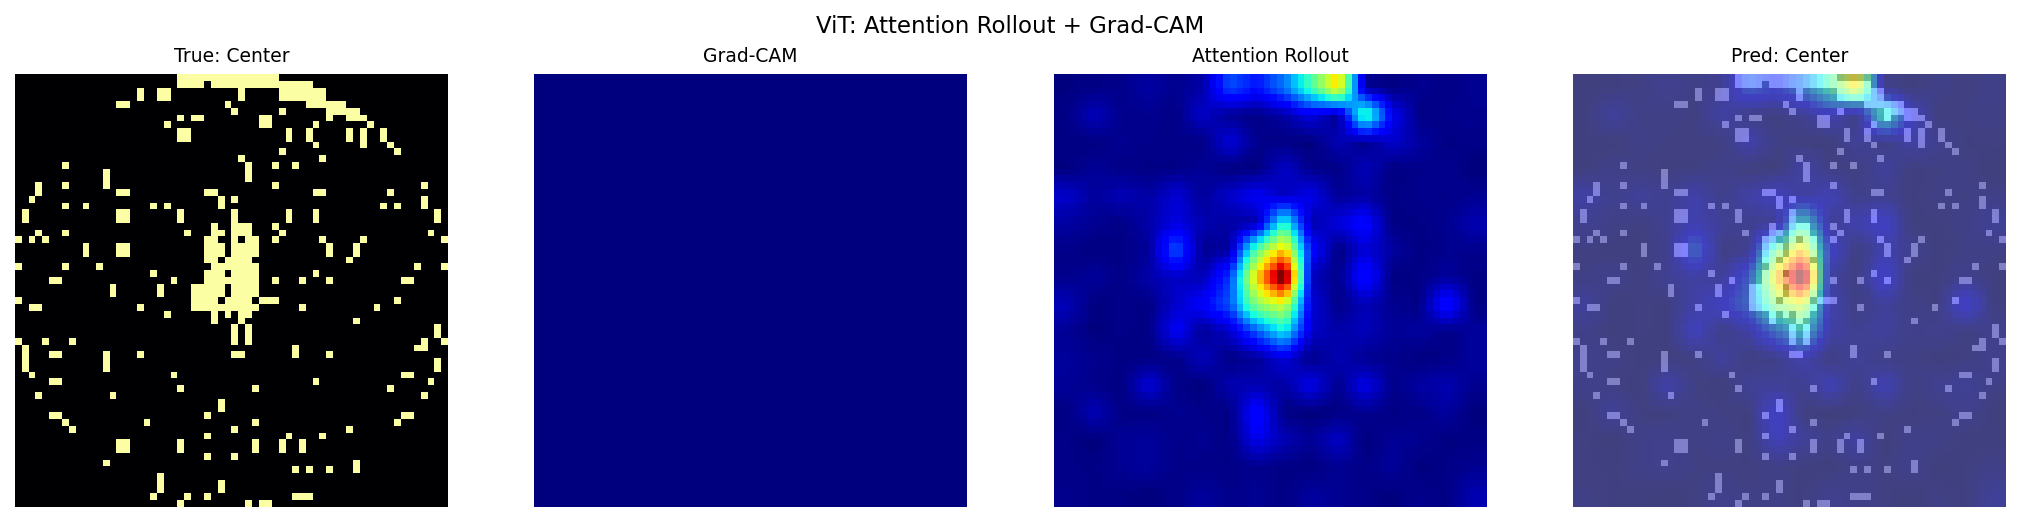
\includegraphics[width=0.98\linewidth]{fig_05.png}
\caption{\textbf{图 4c.} ViT-Tiny —— Center 类解释。从左至右：原始晶圆、Grad-CAM（空白，对非 CNN 架构符合预期）、Attention Rollout 热图、预测叠加图。Rollout 将激活集中于中心缺陷簇，与原生读出假设一致：解释源自模型的前向传播注意力通路，并在该样本中与缺陷模式空间对齐}
\end{figure}

\begin{figure}[htbp]
\centering
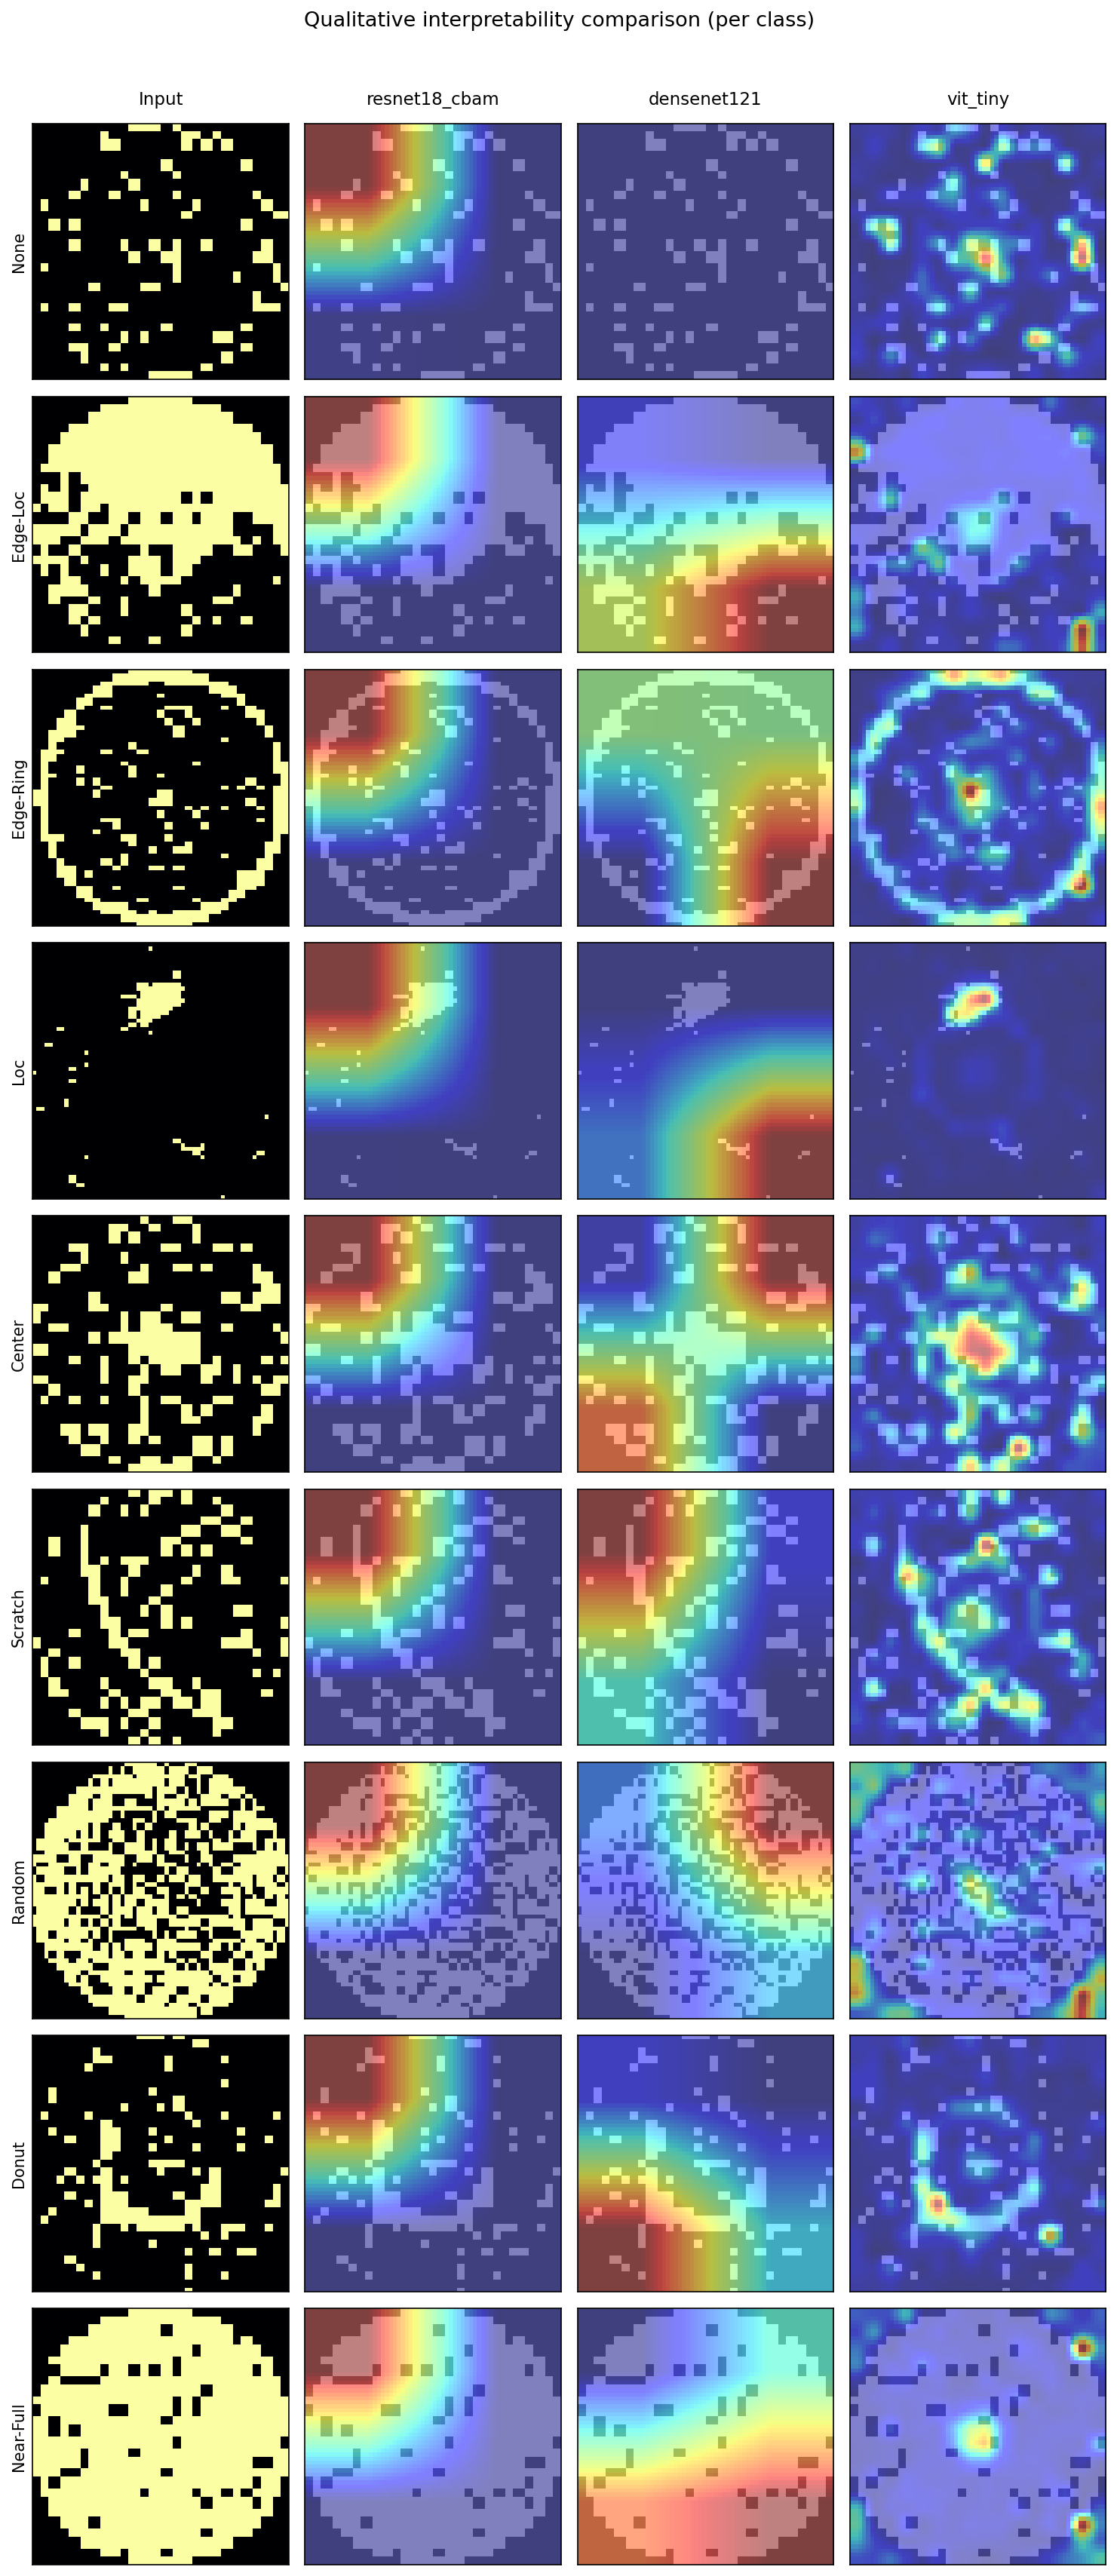
\includegraphics[width=0.60\linewidth]{fig_06.png}
\caption{\textbf{图 5.} 定性热图比较（每类选取置信度最高且分类正确的样本）}
\end{figure}

注意：图 4a–4c 与图 5 使用的样本不同（放大图取自各运行中首个 分类正确的测试样本，而面板选取跨种子置信度最高的样本）。图 4a 展示了 ResNet18+CBAM 的一种退化 Grad-CAM 情形——在某些输入上 并不罕见——而面板则呈现更常见的象限锁定模式。（退化热图产生于 ReLU 后梯度加权激活对目标类别的正质量接近零时；此时最大最小 归一化无法恢复有意义的空间排序。）

尽管三种方法在相同数据与相同优化协议下训练出的模型上运行，其 解释在定性上仍呈现显著差异。关于图 5 的一点说明：该图将各方法 的热图\textbf{半透明叠加}在输入晶圆上显示，这种叠加可能将热图本身的 行为与晶圆背景的空间结构视觉上混淆。去除晶圆背景、并让各热图 按自身动态范围归一化后的\textbf{原始热图}见补充图 S2——该图更清晰地 展现了每种方法的内在行为。

ResNet18+CBAM 的 Grad-CAM 产生的热图范围较宽、变化平滑，并 \textbf{在本质上与输入无关}：原始视图（补充图 S2）显示，全部九个类别 的晶圆上都出现近乎相同的左上角红色色块，仅在强度等高线上有 微小差异。叠加图中看似与类别相关的结构主要来自晶圆背景透过近乎固定的 Grad-CAM 色块显现出来，因此该热图更像粗粒度的象限级激活模式，而不是具备形状感知能力的缺陷定位。

DenseNet121 的 Grad-CAM 在空间 范围上与前者相当，但把高亮放在不同的、且同样\textbf{大致与输入无关} 的区域：多数类别都吸引出一个右下或左下的色块，同样未能勾勒 缺陷几何。对同一张输入而言，两种 Grad-CAM 很少在象限上达成 一致 —— 尽管二者对应的模型取得了几乎相同的分类准确率 （balanced accuracy ≈ 0.901）。这种\textbf{与架构相关}的分歧颇具启示：它说明 Grad-CAM 报告的是各模型特有的梯度路径，而非唯一的真值显著性； CNN 对某个区域“看似专注”的表现，主要是其已学习到的滤波器 统计性质，而非输入本身的属性。

这一定性印象被定量证据所佐证：通过计算热图与晶圆缺陷像素 分布之间的 Spearman 秩相关（补充表 S4），ResNet18+CBAM 的 平均相关系数为 0.037 ± 0.105，DenseNet121 为 0.015 ± 0.126—— 两者在统计上与零无法区分；而 ViT-Tiny 达到 0.318 ± 0.209， 约为 CNN 家族的 8–21 倍。换言之，两种 Grad-CAM 几乎不携带 任何关于缺陷位置的空间信息，而 Attention Rollout 则携带可测量 （虽然带有噪声）的空间信号。

ViT-Tiny 的 Attention Rollout 则与两个 CNN 家族形成对照：它不勾勒大面积区域，而是产生\textbf{稀疏、 高对比度的热点}，且热点位置\textbf{随输入有意义地变化}（见补充图 S2）。 与缺陷的空间对应在具有\textbf{紧致、几何上具有显著特征}的类别上最为 明显：\textbf{Center} 的主要热点直接落在中心缺陷簇上，\textbf{Loc} 的热点 对准局部缺陷簇，\textbf{Edge-Ring} 的热点则沿环形结构本身分布—— 覆盖整个圆周，而非集中于某一段弧线。在其他类别上，对应关系 较弱：\textbf{Donut} 的热点虽有分布但未能清晰勾勒环形；\textbf{Edge-Loc} 的热点部分地跟踪了边缘，但也有相当一部分落在目标之外； \textbf{Near-Full} 即便缺陷接近全局，仍出现一个中心热点。对于 \textbf{None}，热图缺乏连贯的缺陷形状结构，这符合不存在标注缺陷信号的预期。对于 \textbf{Random}， 热点散布在晶圆上而未跟踪弥散的缺陷像素，但其激活模式在视觉上 仍可与 None 区分——人工审核者可以利用这种对比，即使方法本身 未能定位缺陷。\textbf{Scratch} 则部分跟踪了弧形缺陷轨迹，在空间 对齐上表现优于 Edge-Loc，尽管该模式本身是细粒度的。此外，多数类别上在晶圆的圆形边缘附近都出现一组反复 出现的边界热点，这可能反映了模型在关注背景/晶圆过渡区而非 类别相关证据。关键在于，即便 ViT-Tiny 的空间定位并不完美，其 \textbf{逐样本}的热点模式仍随输入变化，这与两种 Grad-CAM 在象限 锁定、基本与类别无关的行为在定性上截然不同。这种细粒度定位视觉上十分 令人信服，然而如 §4.1 所示，ViT-Tiny 的 macro-F1 仍比任一 CNN 家族低约 10 个百分点 —— 这带出本文的核心问题：ViT 的热图究竟 是忠实地反映了它（较弱的）决策，还是仅仅比 CNN 的热图更好看？ §4.3
的定量忠实度分析将回答这一问题。


\subsection{定量忠实度（整体）}

§3.4.3 中定义的三个忠实度指标在表 4 中报告，每家族在 594 个 样本上取均值（每种子 200 个均衡分层采样样本 × 3 个种子）。ViT-Tiny 配合 Attention Rollout 取得最低（最忠实）的 Deletion AUC —— 不到任一 CNN 家族的一半——并且相应地取得最高的 Insertion AUC。Stability 在各家族均值上相当（0.834–0.891），但 ViT-Tiny 的分布最紧凑（标准差 0.107，而 CNN 家族为 0.258–0.275）。

\begin{table}[htbp]
\centering
\small
\caption{\textbf{表 4.} 定量忠实度指标（均值 ± 标准差，n=594）}
\resizebox{\linewidth}{!}{%
\begin{tabular}{lrrrrr}
\toprule
家族 & 运行数 & 样本数 & Deletion AUC ↓ & Insertion AUC ↑ & Stability ↑ \\
\midrule
ResNet18+CBAM & 3 & 594 & 0.495 ± 0.270 & 0.534 ± 0.247 & 0.834 ± 0.275 \\
DenseNet121 & 3 & 594 & 0.525 ± 0.286 & 0.511 ± 0.268 & 0.891 ± 0.258 \\
ViT-Tiny & 3 & 594 & 0.211 ± 0.233 & 0.693 ± 0.274 & 0.845 ± 0.107 \\
Swin-Tiny & 3 & 594 & 0.432 ± 0.233 & 0.480 ± 0.222 & 0.893 ± 0.097 \\
\bottomrule
\end{tabular}
}
\end{table}

图 6 展示了按热图排名逐步移除（deletion）或加入（insertion） 像素时，预测类别的平均概率变化。ViT-Tiny 的 deletion 曲线在前 20\% 像素被移除时就迅速下降，到 40\% 时已降至接近随机的水平， 这表明 Attention Rollout 将重要度集中在一组紧凑的预测相关像素上。 两个 CNN 家族则下降更为平缓，说明其 Grad-CAM 热图把重要度 分散到一片包含大量非关键像素的较大区域。在 insertion 侧， ViT-Tiny 只需插入 40\% 的像素即可恢复超过 60\% 的置信度，而两个 CNN 家族几乎需要全部像素才能达到相当的置信度。


\begin{figure}[htbp]
\centering
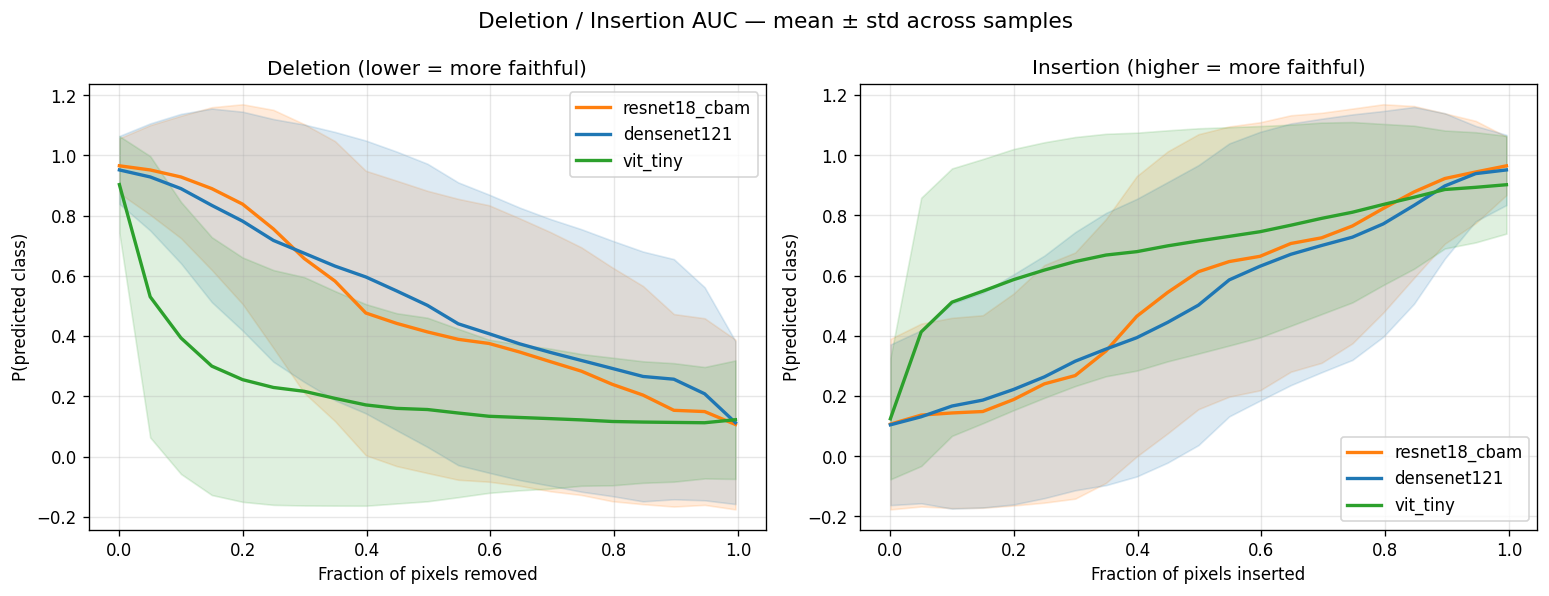
\includegraphics[width=0.98\linewidth]{fig_07.png}
\caption{\textbf{图 6.} Deletion 与 Insertion 曲线（在 594 个样本上的均值 ± 标准差）}
\end{figure}

逐样本的稳定性 —— 即在 §3.4.3 定义的 $K{=}5$ 种语义保持扰动下， 热图两两之间的余弦相似度 —— 以箱线图形式展示于图 7。DenseNet121 取得最高的中位稳定性（约 0.99），但其分布最宽，且在零附近 聚集了一批离群点。这些离群点主要对应 “None” 类样本，在这类 样本上 Grad-CAM 会产出退化的全零热图；一旦出现这种退化，任何 轻微扰动都会产生本质上毫不相干的热图，使得余弦相似度塌缩至 零。ResNet18+CBAM 呈现与此类似的情形：中位值很高但伴有少量 因相同退化机制引起的低稳定性离群点。ViT-Tiny 则表现出另一种 特征：其中位稳定性稍低（约 0.93），但四分位距显著更紧 （标准差 0.107，而 CNN 家族为 0.258–0.275），表明其解释在 所有类别（包括 “None” 类）上都一致稳健 —— 因为 Attention Rollout 总能在 patch 上给出非平凡分布。

另一种诠释也值得指出：在非退化样本上，DenseNet 的高稳定性 可能表明其 Grad-CAM 热图虽然在 Deletion 意义上不忠实，但至少 是 \emph{一致地} 不忠实 —— 总是高亮相同的、与预测无关的区域。 一个等价的解释是：ViT-Tiny 较低的稳定性反映了其与缺陷位置更 紧密的耦合——增强操作移动了缺陷像素，热图也随之移动；而 CNN 热图之所以稳定，恰恰是因为它们对实际驱动预测的空间细节 不敏感。因此稳定性本身并不等同于忠实度，必须与上文的 Deletion 和 Insertion 指标结合来解读。


\begin{figure}[htbp]
\centering
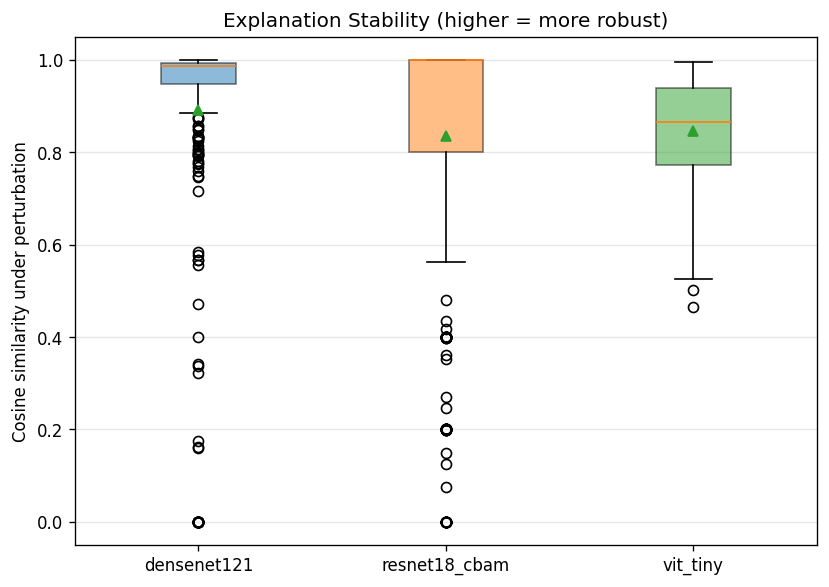
\includegraphics[width=0.60\linewidth]{fig_08.png}
\caption{\textbf{图 7.} 解释稳定性分布（K=5 种扰动下的逐样本余弦相似度）}
\end{figure}

这一结果更适合解读为复合架构--解释器距离的证据。读出直接性与空间粒度在四个家族间并非完全独立：ViT-Tiny 在两个维度上都更接近原生读出，Swin-Tiny 居中，而两个 CNN 家族在两个维度上都更远。ViT Grad-CAM 消融（§S9）和最后层 CLS 注意力消融（§S10）提供了部分分解，表明原生注意力的直接访问与多层 Rollout 深度都对观察到的差距有实质贡献。


\subsection{按类别拆分、效应量与 Bootstrap 置信区间}

上文的整体家族层面比较仅用三个数字概括每一项指标。本小节将 同一批测量沿两个维度 —— 九个缺陷类别与 bootstrap 重采样副本 —— 进行拆分，以判断原生读出优势是数据集整体的属性，还是某个有利 子集的伪影。

表 5 给出每个（家族，类别）组合的平均 Deletion AUC。ViT-Tiny 在 \textbf{九个类别中的八个} 都取得最低（最忠实）的 Deletion AUC， 唯一例外是 \emph{Near-full} 类 —— 在该类别中缺陷几乎覆盖整个晶圆， 忠实度指标对所有家族都趋于退化。在该类上 DenseNet121 取得最低的 Deletion AUC（0.151），从机制上也可以预期：当缺陷在晶圆上空间 均匀分布时，Grad-CAM 的粗感受野不再是劣势，因为本就没有细粒度 的空间结构可供刻画。这种按类别保持的一致性难以归因于噪声： 若原生读出优势仅存在于整体层面，本应看到其排序在多个单独类别上 发生反转。

表 6 报告了家族层面 Deletion AUC 的合并效应量与 95\% bootstrap 置信区间。ViT-Tiny 与任一 CNN 家族之间的 Cohen's \emph{d} 绝对值均 超过 1.1，按惯例这被解释为 \emph{非常大} 的效应。通过对每家族 594 个逐样本测量重采样 2,000 次得到的 95\% bootstrap 置信区间完全 不重叠：ViT-Tiny 位于 [0.192, 0.231]、Swin-Tiny 位于 [0.413, 0.450]、ResNet18+CBAM 位于 [0.474, 0.515]、DenseNet121 位于 [0.502, 0.548]。因此，ViT-Tiny 与三个 Grad-CAM 家族在所评估样本池层面上均可分辨。Swin-Tiny 也与两个 CNN 家族可分辨，但仍明显更接近 CNN 家族而非 ViT-Tiny，这与其中间读出结构位置一致。由于 594 个测量嵌套在仅三个训练种子中，这些 bootstrap 区间应被解释为对所评估样本池的不确定性，而非对独立训练群体的实验级不确定性的完整估计；补充表 S5 中报告的种子级均值提供了互补的种子级视角。

最后，还需要回应一个担忧：整体结果是否由比例过高的 “None” 类 驱动（均衡分层采样下每家族有 66 个 “None” 类样本，共 594 个）。 剔除所有 “None” 类样本后重新计算的 Deletion AUC 均值为： ViT-Tiny 0.163，ResNet18+CBAM 0.466，DenseNet121 0.482。家族 排序保持不变，且 ViT-Tiny 相对两个 CNN 家族的优势幅度与全样本 结果相当（在缺陷类上约 0.30 vs 全样本上约 0.28–0.31）。因此， 该整体效应并非多数类所造成的伪影。


\begin{table}[htbp]
\centering
\small
\caption{\textbf{表 5.} 各类别 Deletion AUC（越低越忠实）。ViT-Tiny 在 9 个类别中的 8 个上最为忠实}
\resizebox{\linewidth}{!}{%
\begin{tabular}{lrrrrrrrrr}
\toprule
家族 & None & Edge-Loc & Edge-Ring & Loc & Center & Scratch & Random & Donut & Near-Full \\
\midrule
DenseNet121 & 0.873 & 0.712 & 0.641 & 0.745 & 0.476 & 0.428 & 0.318 & 0.384 & 0.151 \\
ResNet18+CBAM & 0.719 & 0.644 & 0.762 & 0.548 & 0.367 & 0.596 & 0.309 & 0.312 & 0.195 \\
Swin-Tiny & 0.609 & 0.428 & 0.553 & 0.619 & 0.411 & 0.440 & 0.282 & 0.357 & 0.190 \\
ViT-Tiny & 0.593 & 0.157 & 0.094 & 0.246 & 0.073 & 0.348 & 0.105 & 0.091 & 0.189 \\
\bottomrule
\end{tabular}
}
\end{table}

\begin{table}[htbp]
\centering
\small
\caption{\textbf{表 6.} 所评估样本池上 Deletion AUC 的 95\% bootstrap 置信区间（2,000 次重采样）与 Cohen's \emph{d}。由于样本嵌套在三个训练种子中，这些区间描述的是样本池层面的不确定性，而非完整的实验级不确定性。$|d| > 1.1$ 表明效应量很大}
\begin{tabular}{lrrrr}
\toprule
家族 & Del AUC 均值 & 均值（排除 None） & 95\% CI & n \\
\midrule
ViT-Tiny & 0.211 & 0.163 & [0.192, 0.231] & 594 \\
Swin-Tiny & 0.432 & 0.410 & [0.413, 0.450] & 594 \\
ResNet18+CBAM & 0.495 & 0.466 & [0.474, 0.515] & 594 \\
DenseNet121 & 0.525 & 0.482 & [0.503, 0.548] & 594 \\
\bottomrule
\end{tabular}
\end{table}

\begin{Verbatim}
Cohen d (ViT vs Swin-Tiny): 约 -0.95  [大的效应]
Cohen d (ViT vs ResNet+CBAM): -1.13  [非常大的效应]
Cohen d (ViT vs DenseNet121): -1.21  [非常大的效应]
\end{Verbatim}



\subsection{模型无关对照：RISE 在 WM-811K 上的结果}

原生读出假设的第四个预测（§1.2）指出，模型无关解释器应使各家族 的忠实度排序差距大幅压缩。表 7 报告了 WM-811K 上 RISE 与原生方法的 对比。

\begin{center}
\small \textbf{表 7.} WM-811K 上原生方法 vs. RISE 的忠实度（每家族主种子：Swin-Tiny 使用 seed 7，其他家族使用 seed 42；n=198 样本）。Deletion AUC：越低越忠实；Insertion AUC：越高越忠实
\end{center}

\begin{tabular}{lcccc}
\toprule
家族 & 原生 Del ↓ & RISE Del ↓ & 原生 Ins ↑ & RISE Ins ↑ \\
\midrule
ResNet18+CBAM & 0.486 & \textbf{0.091} & 0.531 & \textbf{0.858} \\
DenseNet121 & 0.544 & \textbf{0.130} & 0.501 & \textbf{0.823} \\
Swin-Tiny & 0.432 & \textbf{0.096} & 0.480 & \textbf{0.823} \\
ViT-Tiny & \textbf{0.221} & \textbf{0.093} & \textbf{0.689} & \textbf{0.818} \\
\bottomrule
\end{tabular}


结果值得注意：RISE 将 Deletion AUC 的分布范围从 0.221–0.544 （原生方法）压缩至 0.091–0.130（RISE）——大幅压缩家族间差距。在原生 方法下，ViT-Tiny 以 Del 0.221 占优；在 RISE 下，四个家族均达到 Del < 0.13，家族间差距相较原生方法大幅压缩。这与第四个预测一致：原生方法 观察到的忠实度差距主要来自 \emph{解释器通路}，而非架构学习表征本身。当解释器在各架构间保持一致（均为 RISE）时，原生方法的忠实度差距大幅缩小，各架构在该 WM-811K 协议下呈现出相似的 RISE 可探测性。Swin-Tiny 的 RISE 表现（Del 0.096）与 ViT-Tiny（0.093）和ResNet18+CBAM（0.091）几乎相同，表明其中间水平的原生方法Deletion AUC（0.432）可归因于 Grad-CAM 解释器通路，而非其学习表征的固有局限。需注意 Swin 相对 CNN 的优势具有指标依赖性：Deletion AUC 改善（0.432 vs 0.495–0.525），但 Insertion AUC 未改善（0.480 vs 0.511–0.534），表明 Swin 的空间层级对像素移除敏感性的提升大于对像素插入恢复的提升。

值得注意的是，RISE 在该协议下的扰动忠实度优于任何原生方法（Del 0.09 vs 原生最佳 0.22）。这并不矛盾——它表明 RISE 通过直接探测模型的 输入–输出函数，能够识别梯度或注意力读出遗漏的决策相关像素。 假设关注的是各家族间的 \emph{相对} 排序，而非绝对性能。

从实用角度看，若唯一目标是最大化基于扰动的忠实度且计算成本可接受，RISE（每样本 4,000 次前向传播）可作为更强但更昂贵的离线审计参考。原生读出在以下情况仍有意义：(i) 计算预算有限（Rollout 仅需一次前向传播 vs. RISE 的 4,000 次），(ii) 需要为面向操作员的交互式复核快速生成解释，或 (iii) 目标是理解 \emph{为何} 忠实度在不同架构–解释器配对间变化，而非仅仅最大化忠实度。


\subsection{扰动基线敏感性}

前述 WM-811K 结果使用零填充作为扰动基线——这是领域驱动的选择， 因为晶圆图是稀疏离散芯粒状态数组，零值对应背景/非晶圆值。为 检验家族排序是否对该选择稳健，本文使用高斯模糊填充（σ=3.0） 替代零填充，重复原生方法的 Deletion 评估。

\begin{center}
\small \textbf{表 8.} 零填充 vs 模糊填充 Deletion AUC（WM-811K，每家族主种子，n=198）
\end{center}

\begin{tabular}{lcc}
\toprule
家族 & 零填充 Del ↓ & 模糊填充 Del ↓ \\
\midrule
ViT-Tiny (Rollout) & \textbf{0.221} & 0.693 \\
Swin-Tiny (Grad-CAM) & 0.440 & 0.700 \\
ResNet18+CBAM (Grad-CAM) & 0.486 & \textbf{0.559} \\
DenseNet121 (Grad-CAM) & 0.544 & 0.681 \\
\bottomrule
\end{tabular}

在模糊填充下，ViT 优势消失且家族排序发生显著变化：ResNet18+CBAM 变为最优，而 ViT-Tiny 与 Swin-Tiny 成为两个最弱的家族，其中 Swin-Tiny 以很小差距在数值上最差（0.700 vs. 0.693）。所有家族收敛至较窄范围（0.56–0.70）。因此，Swin-Tiny 在零填充下的中间位置（0.440）在模糊填充下转移到排序底部，说明对填充算子的敏感性并不限于全局注意力 ViT。这表明零填充下 ViT 的优势部分来自稀疏 patch 级热图与零填充算子之间的相互作用；零填充会完全移除局部证据，而不是对其进行平滑。

该结果并不否定原生读出假设，而是限定其适用范围：该假设预测的是指定扰动协议下的相对忠实度。对于离散晶圆图，零填充是主要的、领域驱动的证据移除操作，因为将选定像素替换为背景值可以近似移除局部芯粒状态证据。模糊填充则测试了另一种扰动语义：它不是直接移除证据，而是利用邻域像素平滑被选区域；对于紧凑的缺陷簇，这种操作可能部分重建或保留局部缺陷信号。因此，像 ViT Rollout 这样稀疏且定位准确的热图在模糊填充下反而可能被“惩罚”：其 top-ranked 像素被模糊邻域替换后，模型仍可能保留足够的缺陷证据，导致置信度下降较小、Deletion AUC 变差。因而，模糊填充敏感性说明扰动式忠实度依赖填充算子，填充方式应作为审计协议的一部分报告。

\subsection{边界条件研究：MVTec AD（探索性）}

MVTec AD 作为探索性边界条件研究，而非完全匹配的复制或泛化证明：模型在 ImageNet 上预训练，任务为二分类（缺陷 vs 良品），且仅评估单一种子。因此，该结果用于识别 WM-811K 发现需要限定的条件，而非声称同一排序可直接迁移到所有工业异常检测场景。

\subsubsection{分类性能}

表 9 报告了 MVTec AD 上的分类性能（二分类：正常 vs. 缺陷）。

\begin{center}
\small \textbf{表 9.} MVTec AD 分类性能（seed 42）
\end{center}

\begin{tabular}{lccc}
\toprule
家族 & 准确率 & 平衡准确率 & F1（宏平均） \\
\midrule
DenseNet121 & 0.970 & 0.944 & 0.957 \\
Swin-Tiny（预训练） & 0.963 & 0.937 & 0.947 \\
ResNet18+CBAM & 0.955 & 0.919 & 0.935 \\
ViT-Tiny（预训练） & 0.917 & 0.872 & 0.881 \\
\bottomrule
\end{tabular}


所有家族均达到强分类性能。三个空间层级模型（DenseNet、Swin、 ResNet）聚集在 92–94\% 平衡准确率，而全局注意力模型（ViT-Tiny） 较低（87\%）。值得注意的是，Swin-Tiny——作为 Transformer——与 CNN 表现相当，确认其层级结构为该任务提供了充分的归纳偏置。该性能差距 作为混淆因素在局限性一节（§5.7）中予以讨论。

\subsubsection{可解释性：原生方法 vs. RISE}

表 10 报告了 MVTec AD 上的忠实度指标（200 个缺陷测试样本， seed 42）。IoU 基于像素级真值缺陷掩码计算。

\begin{center}
\small \textbf{表 10.} MVTec AD 可解释性（seed 42，n=200）。IoU 基于真值掩码
\end{center}

\noindent\resizebox{\linewidth}{!}{%
\begin{tabular}{lcccccc}
\toprule
家族 & 原生 Del ↓ & RISE Del ↓ & 原生 Ins ↑ & RISE Ins ↑ & 原生 IoU ↑ & RISE IoU ↑ \\
\midrule
ResNet18+CBAM & \textbf{0.413} & 0.886 & 0.846 & 0.905 & 0.133 & 0.165 \\
Swin-Tiny & 0.509 & 0.709 & 0.909 & 0.927 & 0.102 & 0.162 \\
DenseNet121 & 0.671 & 0.938 & \textbf{0.944} & 0.937 & 0.141 & 0.206 \\
ViT-Tiny & 0.770 & \textbf{0.656} & 0.855 & 0.792 & \textbf{0.244} & 0.116 \\
\bottomrule
\end{tabular}
}


MVTec 的结果在加入 Swin-Tiny 后呈现清晰模式：

\textbf{(1) 空间层级模型的原生方法优于 RISE。} 对于 ResNet（0.413 vs 0.886）、Swin（0.509 vs 0.709）和 DenseNet（0.671 vs 0.938），原生 Grad-CAM 的 Deletion AUC 均显著低于（优于）RISE。仅 ViT-Tiny 反转该模式（原生 0.770 vs RISE 0.656）。这支持了预测 5： Swin 表现得像 CNN 而非 ViT，因为其空间层级为 Grad-CAM 提供了 兼容的读出路径。

\textbf{(2) RISE 未能压缩。} RISE Deletion AUC 范围为 0.656–0.938—— 分布宽泛且无收敛趋势，与 WM-811K 上所有家族压缩至 Del < 0.13 的情况不同。

\textbf{(3) ViT-Tiny 的真值 IoU 最高（0.244）。} 尽管 Deletion AUC 最差，ViT 的注意力图与实际缺陷像素的重叠度最高。忠实度-对-模型 与忠实度-对-真值之间的这种分离在 §5.4 中讨论。


\subsection{RISE 掩码分辨率消融（MVTec AD）}

为检验 RISE 在 MVTec AD 上的不佳表现是否为掩码分辨率不足的 伪影，在掩码分辨率 16 和 32（单元格分别为 16 px 和 8 px）下 重复评估。

\begin{center}
\small \textbf{表 11.} MVTec AD 上 RISE Deletion AUC 随掩码分辨率的变化（mask\_res=8: n=200；mask\_res=16,32: n=50 样本）
\end{center}

\begin{tabular}{lccc}
\toprule
家族 & mask\_res=8 & mask\_res=16 & mask\_res=32 \\
\midrule
ResNet18+CBAM & 0.886 & 0.893 & 0.839 \\
Swin-Tiny & 0.709 & 0.855 & 0.795 \\
DenseNet121 & 0.938 & 0.960 & 0.939 \\
ViT-Tiny & 0.656 & 0.989 & 0.914 \\
\bottomrule
\end{tabular}


提高掩码分辨率并未改善 RISE 的忠实度——事实上 ViT-Tiny 的性能 反而恶化（0.656 → 0.989，mask\_res=16），Swin-Tiny 也未受益于更高分辨率（0.709 → 0.855，mask\_res=16）。这排除了“仅由掩码分辨率 不足导致”的解释：RISE 在 MVTec AD 上的不佳表现不能仅由粗糙的 8×8 掩码网格解释，尽管其他 RISE 超参数（掩码数量、填充值、 平滑方式）尚未测试。默认 mask\_res=8 与 WM-811K 的 64×64 分辨率 和典型缺陷尺度匹配良好（单元格 = 8 px ≈ 缺陷尺度）；对应的 WM-811K 掩码分辨率消融留待未来敏感性分析。


\section{讨论}

\subsection{原生读出假设的检验}

以下解释针对的是模型–解释器对，而非孤立的模型架构。§1.2 列出的 五个预测现在可以对照 §4.3–4.6 中的测量逐一检验，但需要强调：主要结论是协议条件下的结论。 第一个预测指出：在指定零填充协议下，相比事后近似决策算子的解释，直接从模型决策 算子上读出的解释应得到更低的 Deletion AUC 与更高的 Insertion AUC。ViT-Tiny + Rollout 组合的 Deletion AUC（0.21）不到任一 Grad-CAM 组合（0.43–0.53）的一半，Insertion AUC 的排序也相应 反转（0.693 vs 0.480–0.534），这与预测一致。第二个预测指出：忠实度排序应与 分类排序无关；§5.2 直接证明了这一分离。第三个预测指出：忠实度 排序应在不同随机种子下稳定。逐种子的 Deletion AUC 均值见补充 表 S5；各家族 Deletion AUC 均值的跨种子标准差均低于 0.02 （补充表 S5），家族排序（ViT-Tiny 最忠实，其次 Swin-Tiny，再次 ResNet18+CBAM， DenseNet121 最差）在任一种子上都没有歧义。

第四个预测——模型无关解释器应使忠实度排序趋于一致——得到了 RISE 实验（§4.5）的支持：对所有家族施加同一模型无关解释器后，Deletion AUC 范围从原生方法下的 0.211–0.525 压缩至 0.091–0.130。这表明，在 WM-811K 零填充协议下，原生方法差距主要是解释器通路的属性，而不是各架构是否可被扰动方法探测的差异。

第五个预测——层级 Transformer 应与 Grad-CAM 而非 Attention Rollout 对齐——也得到两个数据集的支持。在 WM-811K 上， Swin-Tiny 的 Grad-CAM Deletion AUC 为 0.432，位于 ViT（0.211） 与 CNN（0.495–0.525）之间，而不是接近 ViT 的 Rollout 表现。 在 MVTec AD 上，Swin 的原生 Grad-CAM 在 Deletion 上优于 RISE （0.509 vs 0.709），与两个 CNN 相同而与 ViT 相反。这说明 Grad-CAM 兼容性的关键因素是 \textbf{空间层级}——即是否存在逐步下采样且 保留空间结构的特征图——而不是卷积/注意力这一架构家族标签。 Swin 在计算意义上完全是 Transformer（自注意力是其唯一计算原语）， 但其层级空间结构使 Grad-CAM 成为兼容的读出方式，正如对 CNN 一样。

Swin-Tiny 的中间位置也符合这一解释：它具有 Transformer 的注意力计算，但保留层级空间特征图，因此在读出结构上更接近 CNN，而不是全局 CLS-token ViT。

两个结构距离代理将该假设操作化。第一个是 \textbf{空间粒度}： ViT-Tiny 以 4×4 patch 分辨率读出重要度（每 token 约占图像的 0.4\%），而 Grad-CAM 通过 \texttt{cbam4} 或 \texttt{denseblock4} 的有效感受野 读出，在远比 4×4 ViT patch 网格粗糙的空间尺度上运作。只能在粗空间尺度上赋予重要度的方法， 在结构上就不可能在 Deletion 扰动中精确移除那些与决策相关的像素。 第二个代理是 \textbf{读出直接性}：Rollout 读取的是构成模型原生信息 路由通路一部分的注意力矩阵，而 Grad-CAM 则从并非为暴露可解释 路由信号而设计的激活的梯度中重建重要度。两个代理都预测了所观察到 的排序，且都与具体训练运行无关 —— 它们是模型–解释器对的架构 属性。

对于将观察到的效应在两个代理之间进行归因，存在一个方法论上的 警示。在本文考察的四个家族中，两个代理在排序上大致正相关： ViT-Tiny 在两个代理上的结构距离都很小（直接读出、细粒度），而两个 CNN 家族在两个代理上的结构距离都很大（间接读出、粗粒度）。 两个针对 ViT 的消融部分解耦了读出直接性与 Rollout 深度，但对空间粒度仅形成间接控制：\textbf{(i) 对 ViT-Tiny 施加 Grad-CAM} （补充表 S7）—— 大致固定空间粒度、加大读出距离 —— 结果 （Del 0.492，与 CNN Grad-CAM 无异）表明读出直接性携带大量信号； \textbf{(ii) ViT-Tiny 的最后一层 CLS 注意力}（补充表 S10）—— 固定 读出来源（原生注意力）、移除多层 Rollout 深度 —— 结果 （Del 0.367 ± 0.031，三种子均值）落在完整 Rollout（0.211）与 ViT Grad-CAM（0.492）之间。两个消融合计将 Rollout-vs-CNN 总差距 （≈0.30）分解为约 42\% 归因于读出直接性、52\% 归因于路径深度， 两个被操控的因素均携带独立信号（残余 ≈6\% 反映两个操作的非可加性； 该分解是路径依赖的）。因此合成结构距离可预测忠实度，且任一 代理都不能单独解释全部效应。

还有一条证据支持将该效应解读为架构性而非噪声驱动。每类别分析 （§4.4）表明 ViT-Tiny 不仅在合并均值上、在 9 个缺陷类别中的 8 个上也都取得最低的 Deletion AUC。合并的效应量 Cohen's \emph{d} 约为 1.1–1.2（相对任一 CNN 家族），且 95\% bootstrap 置信区间 完全不重叠。因此原生读出的优势在样本层面是可分辨的，这与 结构性解释而非统计偶然相一致。

综合来看，上述结果支持审计协议层面的解读，而非普适的解释器排名。WM-811K 零填充结果表明架构–解释器兼容性可以强烈影响扰动忠实度。RISE 结果表明原生读出并非最优性保证：模型无关扰动探测可以达到更强的扰动忠实度，并可作为强有力的离线审计参考。模糊填充敏感性分析进一步表明所测忠实度依赖于扰动算子。因此，工业视觉检测中的解释忠实度应被视为模型–解释器–扰动协议的经验属性。热图不应仅因视觉上合理或架构原生就被部署；它们应在文档化的扰动协议下接受审计，并与模型无关基线进行比较。

\subsection{分类性能 vs. 可解释性}

表 12 将主要分类指标（宏 F1）与两个主要忠实度指标（Deletion AUC 与 Insertion AUC）并列，揭示出模型质量这两个维度之间清晰 的分离。DenseNet121 与 ResNet18+CBAM 的宏 F1 几乎完全相同， 分别为 0.853 与 0.849，Swin-Tiny 为 0.792，而 ViT-Tiny 落后至 0.747。一旦按 Deletion AUC 排序（越低越忠实），顺序便反转过来： ViT-Tiny 取得 0.211，而 Swin-Tiny 为 0.432、ResNet18+CBAM 为 0.495、DenseNet121 为 0.525。Insertion AUC 给出相同的反转排序： ViT-Tiny 为 0.693，领先于 ResNet18+CBAM（0.534）、DenseNet121 （0.511）与 Swin-Tiny（0.480）。因此 CNN 家族主导分类，而全局 注意力 ViT + Attention Rollout 在扰动忠实度上最优。这种分离支持了原生读出 假设（§1.2）的第二个预测：家族间的忠实度排序独立于其分类 排序，因为二者度量的是模型–解释器对结构上独立的属性。

\begin{table}[htbp]
\centering
\small
\caption{\textbf{表 12.} WM-811K 上分类性能与忠实度的对照（宏 F1：3 种子均值；忠实度指标：594 样本汇总）}
\begin{tabular}{lrrr}
\toprule
家族 & 宏 F1 & Deletion AUC ↓ & Insertion AUC ↑ \\
\midrule
DenseNet121 & 0.853 (最佳) & 0.525 (最差) & 0.511 (最差) \\
ResNet18+CBAM & 0.849 & 0.495 & 0.534 \\
Swin-Tiny & 0.792 & 0.432 & 0.480 \\
ViT-Tiny & 0.747 (最差) & 0.211 (最佳) & 0.693 (最佳) \\
\bottomrule
\end{tabular}
\end{table}

\subsection{视觉一致性是否意味着忠实度？}

§4.2 与 §4.3 中汇集的证据表明，视觉上的一致性并不等价于忠实度， 而原生读出框架给出了机制上的解释。定性上，CNN 的 Grad-CAM 热图平滑、看似合理，其宽泛的高亮区域预期应与缺陷区重合；然而定量上，它们 约 0.5 的 Deletion AUC 表明，其中相当比例的高亮像素即使被置零， 对预测也没有实质影响。随机像素基线（补充表 S6）表明 CNN Grad-CAM 排序不优于随机排列（ResNet Del 0.486 vs 随机 0.498；DenseNet Del 0.544 vs 随机 0.508——均处于或高于随机水平），而 ViT-Tiny Rollout（Del 0.221）远高于随机基线（0.480）。ViT-Tiny 稀疏而对比度高的热点虽然缺少 Grad-CAM 输出的 “美感”，但在扰动协议下对预测更关键：移除它们会使模型置信度迅速塌缩。在 原生读出假设下，这一结果是预料之中的。Grad-CAM 之所以外观平滑， 是因为它与 CNN 决策机制在结构上距离较远 —— 梯度加权激活在 空间上是低通的，因此视觉上“好看”；而 Rollout 的稀疏性则是它 与 Transformer 注意力导出的 rollout 图距离近的 \emph{结果} —— 后者在 经验上是集中的，即对任何一个给定预测，只有少数 patch 主导了 [CLS] 的读出。 因此，视觉一致性更适合作为定性诊断，而面向审计的解释主张应由基于扰动的忠实度指标加以支持。

\subsection{跨数据集分析：边界条件}

MVTec AD 的结果（§4.7）表明原生读出假设并非在所有设定下都能 直接迁移。与 WM-811K 的三方面对比需要解释。

\textbf{为何 RISE 在 WM-811K 上压缩但在 MVTec 上失败？} 在 WM-811K 上，四个家族均从头训练于简单几何图案（64×64 灰度）。所得内部 表征结构相当：每个模型都学会检测缺陷像素的空间聚类，RISE 的 随机掩码能有效探测这一共享决策边界。在 MVTec AD 上，模型使用 不同的预训练骨干（CNN vs. Transformer），可能编码了来自 ImageNet 的 实质不同的特征层级。RISE 探测的是模型的实际输入–输出函数，而该 函数在该预训练设定下可能在各架构间存在实质差异；这为缺乏压缩提供了一种合理解释。掩码分辨率消融 （§4.8）削弱了分辨率伪影的解释。

\textbf{为何原生方法的排序反转？} 在 WM-811K 上，ViT-Tiny 的 Attention Rollout 尽管分类性能较弱，却取得了最佳 Deletion AUC；而在 MVTec 上，ResNet18+CBAM 的 Grad-CAM 最优，ViT-Tiny 的 Rollout 则是原生方法中最弱。因此，该反转不太可能仅由准确率差距解释。更合理的解释是，ImageNet 预训练的空间层级骨干更适配 MVTec 中纹理型异常模式和二分类缺陷检测设定，而全局注意力 ViT 的读出与微调后的决策边界对齐较弱。ViT-Tiny 在 MVTec 上较低的准确率（平衡准确率 87\% vs. 三个空间层级模型的 92--94\%）可能放大了这一效应，但更适合被视为伴随因素，而不是主导原因。

\textbf{为何 ViT 的真值 IoU 最高但 Deletion AUC 最差？} Deletion AUC 衡量热图是否识别了 \emph{模型} 依赖的像素；IoU 衡量热图是否与 \emph{实际 缺陷} 重叠。ViT 的注意力图覆盖了缺陷区域（高 IoU）但未精确 排序模型用于决策的像素（高 Deletion AUC）。这表明在 MVTec 上 ViT 的注意力具有空间感知但缺乏决策精确性——与其较低的分类准确率 一致。

综合来看，这些结果表明，原生读出假设在以下条件下最清晰地得到支持：模型具有可比的内部表征，例如在领域特定数据上从头训练；并且解释方法与决策机制之间的结构距离是变异的主要来源。当预训练模型带来实质不同的 特征层级时，架构的表征本身成为主导因素，解释器通路退居次要。Swin-Tiny 的加入使这一综合更为清晰：在 MVTec 上，所有三个空间层级模型（ResNet、DenseNet、Swin）的原生 Grad-CAM 均优于 RISE，而只有全局注意力模型（ViT）反转了该模式。无论空间层级是通过卷积（ResNet、DenseNet）还是窗口自注意力（Swin）实现，该结论均成立，支持关键架构属性是层级空间特征图的存在而非具体计算原语的解释。需要指出的是，MVTec 上的排序反转可由多种解释——包括ViT 在 MVTec 上分类准确率较低（87\% vs. 92--94\%）、预训练领域不匹配、以及任务结构差异——当前数据无法唯一区分这些解释。

最后一层 CLS 注意力消融进一步阐明了 MVTec 上 ViT 的失败模式： 最后一层注意力（Del 0.857）表现劣于完整 Rollout（0.770），表明 多层整合仍然有益。然而两种原生注意力方法均被 RISE（0.656）超越， 说明主要限制并非仅是 Rollout 深度不足。在预训练 MVTec 设定下， 原生注意力矩阵似乎仅部分对齐于微调后的决策边界；RISE 通过直接 探测模型的输入–输出响应绕过了该通路。这与 WM-811K 形成对比： 从头训练似乎产生了与任务特定决策证据更好对齐的注意力矩阵。

这些结果限定了该假设的适用范围，并澄清了在何种条件下解释器通路效应更可能主导表征层面的差异。

\subsection{实用建议}

基于上文所检验的假设，可以给出四点面向部署的建议。第一，选择 解释器时应检查模型的读出结构，而不是仅看架构家族标签。若模型 产生层级空间特征图（CNN 或 Swin 类架构），则最终空间阶段上的 Grad-CAM 是合适的原生方法；若模型使用带 [CLS] token 的全局 注意力（ViT 类架构），则应优先考虑 Attention Rollout。该规则 替代了简单但不充分的“CNN → Grad-CAM，Transformer → Rollout” 启发式。第二，当 向人工操作员呈现解释用于缺陷复核时，相似晶圆之间的“一致性” 通常比“峰值中位表现”更重要；ViT-Tiny 紧凑的稳定性分布（标准差 0.107）以及 Swin-Tiny 较高且稳定的解释一致性（标准差 0.097）使二者在优先考虑解释一致性时成为值得进一步研究的候选方案，尽管其较低的分类准确率在部署前仍需解决。 第三，当解释用于驱动下游自动化 —— 如对可疑区域做掩蔽以进行 复检 —— Deletion 与 Insertion AUC 最为相关；在 WM-811K 零填充协议下，ViT-Tiny 是最强的原生方法候选，而 RISE 则提供更强但更昂贵的离线审计参考。第四，当分类准确率是首要目标、可解释性次之时， DenseNet121 或 ResNet18+CBAM 仍是合适选择，\emph{前提是} 同时 报告相应的忠实度指标，避免对热图含义过度解读。在设计层面， 该假设还提示一条前瞻性原则：用于可解释部署的架构应从一开始 就与其解释通路协同设计，而非临时嫁接一个事后解释器 —— 后者 与决策机制的结构距离可能限制其在给定协议下的测量忠实度。在分类 准确率不可妥协的场景下，原生读出原则启发未来研究探索混合 架构 —— 例如用 CNN 骨干获取分类强度，再用一个轻量级 Transformer 头提供注意力矩阵作为解释读出。

表 13 按部署目标汇总了推荐的审计选择，基于两个数据集的证据。

\begin{center}
\small \textbf{表 13.} 按部署目标推荐的解释器审计选择
\end{center}

\begin{tabular}{lll}
\toprule
部署目标 & 推荐审计选择 & 依据 \\
\midrule
快速定性复核 & 原生解释器 & 低开销，兼容 \\
离线忠实度审计 & RISE & 直接探测输入–输出 \\
晶圆图 ViT 解释 & Attention Rollout & WM-811K 上忠实度强 \\
诊断 ViT 失效 & 最后层 CLS vs Rollout & 分离访问与深度 \\
CNN Grad-CAM 可靠性 & 随机基线 + RISE & 检测不忠实先验 \\
预训练模型检测 & 用 RISE 验证 & 原生可能失配 \\
\bottomrule
\end{tabular}

\subsection{工业视觉检测的实用审计流程}

基于 WM-811K 与 MVTec AD 的结果，我们建议将解释生成视为工业 视觉检测系统中可审计的组件，而非仅作为可视化后处理步骤。 图 8 总结了所提出的流程。

该流程被组织为审计序列，而不是简单的可视化流水线。步骤 [1] 首先明确解释的预期用途，因为模型审计、缺陷定位、人工复核和下游自动化所强调的评价标准并不相同。步骤 [2]--[3] 在进入可解释性分析之前先建立预测性能基线。步骤 [4] 根据模型读出结构选择原生解释路径：空间层级模型进入 Grad-CAM 路径 [4a]，而全局 CLS-token ViT 进入 Attention Rollout 路径 [4b]。步骤 [5]--[6] 使用扰动指标与对照方法审计所得热图，包括随机基线、RISE 以及扰动填充敏感性。若解释主张未能经受这些对照，步骤 [7a] 先诊断失效模式，再在步骤 [8] 中选择带有限定条件的部署策略。
\clearpage
\begin{figure}[htbp]
\centering
\resizebox{0.9\linewidth}{!}{%
\begin{tikzpicture}[
    font=\sffamily\small,
    node distance=9mm and 13mm,
    hand/.style={
        decorate,
        decoration={random steps,segment length=4pt,amplitude=0.25pt}
    },
    arrow/.style={
        -{Stealth[round,length=5pt]},
        draw=black!55,
        line width=0.55pt,
        hand
    },
    box/.style={
        rectangle,
        rounded corners=3pt,
        draw=black!65,
        fill=black!3,
        line width=0.75pt,
        align=center,
        text width=33mm,
        minimum height=8mm,
        inner sep=4pt
    },
    keybox/.style={
        rectangle,
        rounded corners=5pt,
        draw=blue!55!black,
        fill=blue!4,
        line width=0.75pt,
        align=center,
        text width=33mm,
        minimum height=8mm,
        inner sep=4pt
    },
    decision/.style={
        diamond,
        aspect=1.8,
        draw=black!65,
        fill=black!2,
        line width=0.65pt,
        align=center,
        text width=28mm,
        inner sep=2pt
    },
    finalbox/.style={
        rectangle,
        rounded corners=5pt,
        draw=black!75,
        fill=black!5,
        line width=0.75pt,
        align=center,
        text width=35mm,
        minimum height=9mm,
        inner sep=4pt
    }
]

\node[keybox] (use) {[1] 明确用途};
\node[box, below=of use, xshift=0mm] (train) {[2] 训练模型};
\node[box, below=of train, xshift=0mm] (perf) {[3] 评估性能};

\node[decision, below=10mm of perf] (readout) {[4] 读出\\结构？};

\node[keybox, below left=10mm and 14mm of readout] (spatial) {[4a] 空间\\层级};
\node[keybox, below right=10mm and 14mm of readout] (global) {[4b] 全局\\CLS 注意力};

\node[box, below=18mm of readout] (native) {[5] 原生\\解释};
\node[box, below=of native, xshift=0mm] (audit) {[6] 对照\\审计};

\node[decision, below=10mm of audit] (survive) {[7] 主张\\成立？};

\node[box, below left=10mm and 12mm of survive] (diagnose) {[7a] 诊断\\失效模式};
\node[finalbox, below right=10mm and 12mm of survive] (select) {[8] 选择\\策略};

\draw[arrow] (use) -- (train);
\draw[arrow] (train) -- (perf);
\draw[arrow] (perf) -- (readout);

\draw[arrow] (readout) -- node[above left, font=\scriptsize, text=black!60] {Grad-CAM 路径} (spatial);
\draw[arrow] (readout) -- node[above right, font=\scriptsize, text=black!60] {Rollout 路径} (global);

\draw[arrow] (spatial.south) |- (native.west);
\draw[arrow] (global.south) |- (native.east);

\draw[arrow] (native) -- (audit);
\draw[arrow] (audit) -- (survive);

\draw[arrow] (survive) -- node[above left, font=\scriptsize, text=black!60] {否 / 混合} (diagnose);
\draw[arrow] (survive) -- node[above right, font=\scriptsize, text=black!60] {是 / 限定成立} (select);
\draw[arrow] (diagnose.east) |- (select.west);

\end{tikzpicture}
}
\caption{\textbf{图 8.} 面向决策的架构感知解释审计流程。步骤编号在正文中展开说明。}
\end{figure}

\clearpage
\subsection{局限与效度威胁}

有若干局限会影响本文结论的可推广性。本文讨论的结构因素并非完全正交：读出直接性、空间粒度与 Rollout 路径深度在不同模型--解释器配对之间部分共变。在 §1.2 中，原生读出假设主要通过两个代理变量进行操作化，即读出直接性与空间粒度。后续针对 ViT 的消融又引入了第三个因素，即 Rollout 路径深度，因为完整 Attention Rollout 与最后一层 CLS 注意力的差异不仅在于读出来源，也在于信息流跨越多少层被累积。两个消融实验对这些因素进行了部分解耦。对 ViT-Tiny 施加 Grad-CAM（补充表 S7）在固定模型与 patch 级输入粒度的同时扰动读出直接性，得到 Del 0.492，与随机水平无异。最后一层 CLS 注意力（补充表 S10）则将读出来源固定为原生注意力，同时移除多层 Rollout 深度，得到 Del 0.367。综合来看，这些消融表明，对原生注意力的直接访问与多层 Rollout 都对 Rollout 的优势有实质贡献。然而，该分解仍是近似的，因为这些操作并非完全正交：最后一层注意力也改变了层间信息混合的表示方式，而且任一消融都不能将空间粒度作为独立因果因素完全隔离。因此，文中报告的约 42\% / 52\% 划分应被理解为对 WM-811K 所观察差距的一种路径依赖分解，而不是普适的因果归因。

其余局限涉及评估协议与数据集覆盖面。计算 Deletion 与 Insertion AUC 所用的扰动基线是零填充，这在 WM-811K 上是语义合理的 （像素值零编码晶圆背景），但在自然图像的可解释性任务上不能 直接推广，后者更常用模糊或均值填充。此外，将晶圆内部的 die 像素置零可能产生分布外的晶圆图案；因此所报告的 AUC 值 应被解释为在固定扰动算子下的相对比较，而非绝对忠实度分数。 不同基线可能会改变 AUC 的绝对值，并且原则上也可能影响家族间 排序；§4.6 的模糊填充分析已经证明了这一点。64×64 的输入分辨率限制了指标能奖励多细粒度 归因；将实验在 128×128 上重跑可部分控制空间粒度代理。每个 家族仅采用一种代表性解释方法，若将比较扩展到每家族内多种 方法 —— CNN 上的 Grad-CAM++ 或 Score-CAM、Transformer 上 Chefer 等 [10] 的类别特定 LRP + 注意力混合方法，以及像 Khatun 等 [13] 与 Lee 等 [14] 所用的模型无关方法 LIME 与积分梯度 —— 会在读出直接性代理上增加数据点，从而提供更严格的检验。 将忠实度度量与 Lee 等 [14] 示范的温度缩放等概率校准诊断结合 起来，可以得到更完整的部署级解释质量图景。最后，WM-811K 中 “None” 类的主导地位仅被分层采样部分抵消，因此结论对缺陷类最 稳健，对多数类的适用性稍弱。对 top-k 比率（5 \%、10 \%、20 \%） 的敏感性分析表明家族排序对扰动粒度具有鲁棒性（补充表 S12）。由于 bootstrap 置信区间是在三个种子的汇总逐样本测量上计算的，应将 其解读为对所评估样本池的不确定性，而非完全独立的数据集级 不确定性。

关于所观察到的效应，还有两个替代解释需要明确承认。第一， 由于 ViT-Tiny 的宏 F1（0.747）低于任一 CNN 家族（0.849 与 0.853），存在一种可能：较弱的分类器由于其决策边界较简单， 自然会依赖更少、空间上更局域的特征，从而产生稀疏的解释， 这类解释在奖励“稀疏定位”的指标上天然得分较高 —— 与解释方法 是否在结构上特权无关。补充表 S11 直接回应了这一点：仅对三个 家族均正确分类的 140 个样本评估时，排序完全保持（ViT Del 0.216, Swin 0.45, CNN 0.50–0.55），排除了准确率驱动的混淆。第二，WM-811K 上 的零填充 Deletion 协议本身就奖励能够定位缺陷像素的方法，而在 本文使用的 4×4 网格下，patch 级注意力正是在构造上做到这一点； 然而，对 \emph{同一} ViT 模型施加 Grad-CAM（补充表 S7）得到 Del AUC 0.492 —— 与随机无异 —— 证明优势归因于原生读出解释器，而非 ViT 架构或其 patch 粒度。 RISE 实验（§4.5）提供了最直接的判定：RISE 统一应用于四个家族， 将 Deletion AUC 压缩至 0.091–0.130，表明差距归因于解释器通路。 若 RISE 保留了 ViT 的优势，则效应应归因于架构的表征；观察到的 压缩在 WM-811K 扰动协议下削弱了该替代解释。

MVTec AD 边界条件研究（§4.7）引入了第二数据集特有的额外局限。 ViT-Tiny 较低的分类准确率（平衡准确率 87\% vs. 三个空间层级模型的 92--94\%） 是一个无法在缺少匹配 CNN 准确率的 ViT 变体的情况下完全解决的 混淆因素。使用不同预训练骨干（ImageNet CNN vs. ImageNet ViT） 意味着比较测试的是架构 + 预训练的联合效应，而非单独的架构效应。 MVTec 可解释性仅在 seed 42 上评估（不同于 WM-811K 的三种子 协议），因此该数据集上的运行间方差未被表征。RISE 在两个 CNN 家族上表现劣于原生方法（Del 0.886–0.938 vs 原生 0.413–0.671）， 且仅对 ViT-Tiny 有适度改善（Del 0.656 vs 原生 0.770），未能 产生 WM-811K 式的压缩。掩码分辨率消融（§4.8）排除了一种简单 解释，但并未确立 RISE 在 MVTec AD 上已被全局优化（掩码数量、 概率和填充值等其他超参数尚未测试）。

原生读出假设得到了 WM-811K 证据和 RISE 对照的支持，并在 MVTec AD 上识别了边界条件。两个数据集、四个模型家族、两种解释范式（原生 + 模型无关）以及掩码分辨率消融提供了汇聚证据，但不能确立一条普适 原则。§4.6 的模糊填充分析进一步限定了 WM-811K 结论的协议特异性，并说明部署审计中应同时报告扰动基线与忠实度指标。尚待完成的额外消融包括：更大 patch 尺寸的 ViT（P=8，匹配 CNN 空间分辨率， 直接测试粒度代理）、以及 MVTec 上的多种子可解释性评估。本研究的 贡献在于将该假设表述得足够精确，使后续研究得以在其他数据集与 架构–解释器组合上对其进行证伪。

\section{结论}

本文提出了一套架构感知的审计协议，用于评估工业视觉检测中的解释 忠实度。本文不将解释方法视为可互换的事后可视化工具，而是考察 在文档化扰动协议下测得的忠实度是否取决于模型读出结构与所用解释器之间的兼容性。

在 WM-811K 上，结果在零填充扰动协议下支持原生读出假设：ViT-Tiny 搭配 Attention Rollout 取得了最低（最忠实）的原生解释器 Deletion AUC，而 CNN 类模型则与 Grad-CAM 更为匹配。Swin-Tiny 提供了重要 的诊断案例，表明解释兼容性应从读出结构而非宽泛的架构家族来理解： 尽管 Swin 是 Transformer，其层级空间特征图使 Grad-CAM 成为结构 上合适且有竞争力的解释器。与此同时，RISE 在 WM-811K 上优于所有 原生方法，表明原生读出应被理解为兼容性原则而非最优性保证。

额外的敏感性与边界条件分析进一步限定了上述发现。模糊填充敏感性分析进一步表明，Deletion AUC 排序并非解释器的内在属性，而是依赖于审计协议中的扰动算子。探索性 MVTec AD 研究也表明，晶圆图上观察到的趋势不一定直接迁移至异常 检测，后者中数据集结构、预训练、二分类和定位目标均与解释行为 交互作用。

本文并未建立普适的解释器排名。相反，它表明工业视觉检测中的解释可靠性取决于模型架构、解释器读出路径和扰动算子。实践启示在于：不应仅因热图视觉上合理、符合架构惯例，甚至看似架构原生，就直接信任它。解释方法应通过文档化的、架构感知的审计协议来选择和验证；对于面向部署的系统，热图应附带定量扰动忠实度评分、模型无关审计基线以及扰动协议的明确报告。这将解释生成从可视化步骤重新定义为工业 AI 部署中可审计的组件。

\subsection*{参考文献}

\textbf{基础架构与可解释性方法}

\begin{list}{}{\setlength{\leftmargin}{2.5em}\setlength{\labelwidth}{2em}\setlength{\labelsep}{0.3em}\setlength{\itemsep}{0.2ex}}
\item[1.] He, K., Zhang, X., Ren, S., \& Sun, J. \emph{Deep Residual Learning for Image Recognition}. CVPR, 2016. \url{https://www.cv-foundation.org/openaccess/content_cvpr_2016/papers/He_Deep_Residual_Learning_CVPR_2016_paper.pdf}
\item[2.] Woo, S., Park, J., Lee, J.-Y., \& Kweon, I. S. \emph{CBAM: Convolutional Block Attention Module}. ECCV, 2018. \url{https://arxiv.org/abs/1807.06521}
\item[3.] Huang, G., Liu, Z., van der Maaten, L., \& Weinberger, K. Q. \emph{Densely Connected Convolutional Networks}. CVPR, 2017. \url{https://openaccess.thecvf.com/content_cvpr_2017/papers/Huang_Densely_Connected_Convolutional_CVPR_2017_paper.pdf}
\item[4.] Dosovitskiy, A. et al. \emph{An Image Is Worth 16×16 Words: Transformers for Image Recognition at Scale}. ICLR, 2021. \url{https://dblp.org/rec/conf/iclr/DosovitskiyB0WZ21}
\item[5.] Selvaraju, R. R. et al. \emph{Grad-CAM: Visual Explanations from Deep Networks via Gradient-Based Localization}. ICCV, 2017. \url{https://openaccess.thecvf.com/content_ICCV_2017/papers/Selvaraju_Grad-CAM_Visual_Explanations_ICCV_2017_paper.pdf}
\item[6.] Abnar, S., \& Zuidema, W. \emph{Quantifying Attention Flow in Transformers}. ACL, 2020. \url{https://arxiv.org/abs/2005.00928}
\item[7.] Petsiuk, V., Das, A., \& Saenko, K. \emph{RISE: Randomized Input Sampling for Explanation of Black-Box Models}. BMVC, 2018. \url{https://arxiv.org/abs/1806.07421}
\item[8.] Alvarez-Melis, D., \& Jaakkola, T. S. \emph{On the Robustness of Interpretability Methods}. ICML Workshop, 2018. \url{https://arxiv.org/abs/1806.08049}
\item[9.] Jain, S., \& Wallace, B. C. \emph{Attention Is Not Explanation}. NAACL, 2019. \url{https://doi.org/10.48550/arXiv.1902.10186}
\item[10.] Chefer, H., Gur, S., \& Wolf, L. \emph{Transformer Interpretability Beyond Attention Visualization}. CVPR, 2021. \url{https://www.computer.org/csdl/proceedings-article/cvpr/2021/450900a782/1yeIsbbCMO4}
\item[11.] Sundararajan, M., Taly, A., \& Yan, Q. \emph{Axiomatic Attribution for Deep Networks} (Integrated Gradients). ICML, 2017. \url{https://arxiv.org/abs/1703.01365}
\item[12.] Zeiler, M. D., \& Fergus, R. \emph{Visualizing and Understanding Convolutional Networks} (Occlusion sensitivity). ECCV, 2014. \url{https://cs.nyu.edu/~fergus/papers/zeilerECCV2014.pdf}
\end{list}

\textbf{近期晶圆图缺陷分类与 XAI 工作（2024–2026）}

\begin{list}{}{\setlength{\leftmargin}{2.5em}\setlength{\labelwidth}{2em}\setlength{\labelsep}{0.3em}\setlength{\itemsep}{0.2ex}}
\item[13.] Khatun, M. R., Farid, F. A., Dhar, S., Islam, M. S., Uddin, J., \& Abdul Karim, H. \emph{CBAM-Enhanced Lightweight CNN for Wafer Map Defect Classification}. Frontiers in Electronics, 7:1750707, 2026. \url{https://www.frontiersin.org/journals/electronics/articles/10.3389/felec.2026.1750707/full}
\item[14.] Lee, J., Ju, Y., Lim, J., Hong, S., Baek, S.-W., \& Lee, J. \emph{Enhancing Confidence and Interpretability of a CNN-Based Wafer Defect Classification Model Using Temperature Scaling and LIME}. Micromachines, 16(9):1057, 2025. \url{https://www.mdpi.com/2072-666X/16/9/1057}
\item[15.] Lee, C.-Y., Pleva, M., Hládek, D., Lee, C.-W., \& Su, M.-H. \emph{Ensemble Learning for Wafer Defect Pattern Classification in the Semiconductor Industry}. IEEE Access, 13, 2025. \url{https://ieeexplore.ieee.org/iel8/6287639/10820123/11145756.pdf}
\item[16.] Park, S. Y., \& Kim, T. S. \emph{Fuzzy Inference System for Interpretable Classification of Wafer Map Defect Patterns}. Electronics, 15(1):130, 2026. \url{https://www.mdpi.com/2079-9292/15/1/130}
\item[17.] Pilli, V. S. R. R. \emph{Intelligent Model to Detect and Classify Silicon Wafer Map Images}. M.Sc. Thesis, Purdue University, 2024. \url{https://hammer.purdue.edu/ndownloader/files/49412641}
\end{list}

\textbf{基准数据集}

\begin{list}{}{\setlength{\leftmargin}{2.5em}\setlength{\labelwidth}{2em}\setlength{\labelsep}{0.3em}\setlength{\itemsep}{0.2ex}}
\item[18.] Wu, M.-J., Jang, J.-S. R., \& Chen, J.-L. \emph{Wafer Map Failure Pattern Recognition and Similarity Ranking for Large-Scale Data Sets}. IEEE Transactions on Semiconductor Manufacturing, 28(1):1–12, 2015. \url{https://ui.adsabs.harvard.edu/abs/2015ITSM...28S4237W/abstract}
\end{list}

\textbf{边界条件数据集与预训练模型}

\begin{list}{}{\setlength{\leftmargin}{2.5em}\setlength{\labelwidth}{2em}\setlength{\labelsep}{0.3em}\setlength{\itemsep}{0.2ex}}
\item[19.] Bergmann, P., Fauser, M., Sattlegger, D., \& Steger, C. \emph{MVTec AD — A Comprehensive Real-World Dataset for Unsupervised Anomaly Detection}. CVPR, 2019. \url{https://openaccess.thecvf.com/content_CVPR_2019/papers/Bergmann_MVTec_AD_--_A_Comprehensive_Real-World_Dataset_for_Unsupervised_Anomaly_CVPR_2019_paper.pdf}
\item[20.] Touvron, H., Cord, M., Douze, M., Massa, F., Sablayrolles, A., \& Jégou, H. \emph{Training Data-Efficient Image Transformers \& Distillation Through Attention} (DeiT). ICML, 2021. \url{https://arxiv.org/abs/2012.12877}
\end{list}

\textbf{可信工业 AI}

\begin{list}{}{\setlength{\leftmargin}{2.5em}\setlength{\labelwidth}{2em}\setlength{\labelsep}{0.3em}\setlength{\itemsep}{0.2ex}}
\item[21.] Breque, M., De Nul, L., \& Petridis, A. \emph{Industry 5.0: Towards a Sustainable, Human-Centric and Resilient European Industry}. European Commission, Directorate-General for Research and Innovation, 2021. \url{https://op.europa.eu/publication/manifestation_identifier/PUB_KIBD20021ENN}
\item[22.] Moosavi, S., Farajzadeh-Zanjani, M., Razavi-Far, R., Palade, V., \& Saif, M. \emph{Explainable AI in Manufacturing and Industrial Cyber–Physical Systems: A Survey}. Electronics, 13(17):3497, 2024. \url{https://www.mdpi.com/2079-9292/13/17/3497}
\end{list}

\textbf{层级视觉 Transformer}

\begin{list}{}{\setlength{\leftmargin}{2.5em}\setlength{\labelwidth}{2em}\setlength{\labelsep}{0.3em}\setlength{\itemsep}{0.2ex}}
\item[23.] Liu, Z., Lin, Y., Cao, Y., Hu, H., Wei, Y., Zhang, Z., Lin, S., \& Guo, B. \emph{Swin Transformer: Hierarchical Vision Transformer using Shifted Windows}. ICCV, 2021. \url{https://arxiv.org/abs/2103.14030}
\end{list}


\clearpage
\appendix
\phantomsection
\section*{补充材料}
\addcontentsline{toc}{section}{补充材料}

\phantomsection
\subsection*{S1. 实验工作流}
\addcontentsline{toc}{subsection}{S1. 实验工作流}

完整流水线从原始数据摄入到最终报告共分四个阶段，每阶段由 专用脚本自动完成。WM-811K 可通过 \texttt{bash rerun\_report\_journal\_zh.sh} 复现；MVTec AD 可通过 \texttt{python main\_mvtec.py} 及 \texttt{python interpret\_eval\_mvtec.py} 复现。

\begin{Verbatim}
+--------------+     +------------------+     +----------------------+
|  LSWMD.pkl   |---->|  预处理          |---->|  按批次分组划分      |
| (811K 样本) |     |  64x64, nan->0    |     |  70 / 15 / 15        |
+--------------+     +------------------+     +----------+-----------+
                                                         |
                     +-----------------------------------+|
                     |  训练（WM-811K 共 12 次；MVTec AD 共 4 次）||
                     |  4 家族 x 3 种子（WM-811K）
                     |  4 家族 x 1 种子（MVTec AD，seed 42）  |<+
                     |  Adam/AdamW . 余弦 LR . AMP       |
                     |  早停：家族特定验证指标           |
                     |  （bal-acc 或 macro-F1）           |
                     +---------------+-------------------+
                                     |
                     +---------------v-------------------+
                     |          分类评估                  |
                     |  Acc, 平衡 Acc, 宏 F1, MCC         |
                     +---------------+-------------------+
                                     |
                     +---------------v-------------------+
                     |         可解释性评估               |
                     |  每种子 200 个均衡分层样本 x 3 种子   |
                     |  Del AUC . Ins AUC . Stability    |
                     +---------------+-------------------+
                                     |
                     +---------------v-------------------+
                     |           报告生成                 |
                     |  报告 -> HTML + 保存图像           |
                     +-----------------------------------+
\end{Verbatim}

\begin{center}
\small \textbf{补充示意图 S1.} 端到端实验流水线（图中展示 WM-811K 主流程；MVTec AD 使用平行流程）
\end{center}

\clearpage
\phantomsection
\subsection*{S2. 代码结构}
\addcontentsline{toc}{subsection}{S2. 代码结构}

\begin{Verbatim}
+-----------------------------------------------------------------+
|                        CLI 入口脚本                              |
+----------+--------------+------------------+--------------------+
| main.py  | compare.py   | interpret_eval.py| generate_panel.py  |
+----+-----+------+-------+-------+----------+--------------------+
     |            |               |
     v            v               v
+-----------------------------------------------------------------+
|                          src/                                    |
+------------+------------+--------------+------------------------+
| dataset.py | models.py  |  train.py    | interpretability.py    |
| 加载/划分  | 模型注册表 | AMP/LR/Ckpt  | 热图/Del/Ins/Stab      |
+------------+------------+--------------+------------------------+
     |                                          |
     v                                          v
+-----------------------------------------------------------------+
|                         utils/                                   |
+------------------+------------------+---------------------------+
| metrics.py       | visualize.py     | augmentation.py           |
| FocalLoss/Eval   | GradCAM/Rollout  | 旋转/翻转/噪声            |
+------------------+------------------+---------------------------+
\end{Verbatim}

\begin{center}
\small \textbf{补充示意图 S2.} 模块依赖图
\end{center}

代码库遵循四条设计原则。第一，所有实验都是 \textbf{由配置驱动}： 全部超参数都存放在 YAML 文件中，源码中不含魔法数字，任何 运行都可从其保存的配置精确重建。第二，\texttt{src/models.py} 中 采用 \textbf{注册表模式}，通过 \texttt{MODEL\_REGISTRY} 将字符串名称映射到 模型类。第三，在数据层采用 \textbf{按批次分组划分}，以防止同批次 晶圆共享系统性缺陷所引起的信息泄露。最后，项目保持 \textbf{严格的 关注点分离}：训练、评估与可解释性分别位于独立模块中。

MVTec AD 的边界条件研究使用平行的流水线结构：\texttt{main\_mvtec.py}、 \texttt{interpret\_eval\_mvtec.py} 与 \texttt{rise\_eval.py} 分别对应训练、 可解释性评估与 RISE 对照，其数据集与模型模块由 \texttt{dataset\_mvtec.py} 与 \texttt{models\_mvtec.py} 实现，配置文件位于 \texttt{configs\_mvtec/}。

\phantomsection
\subsection*{S3. 训练曲线}
\addcontentsline{toc}{subsection}{S3. 训练曲线}

各家族在 seed 42 下的训练与验证损失曲线见补充图 S1。


\begin{figure}[htbp]
\centering
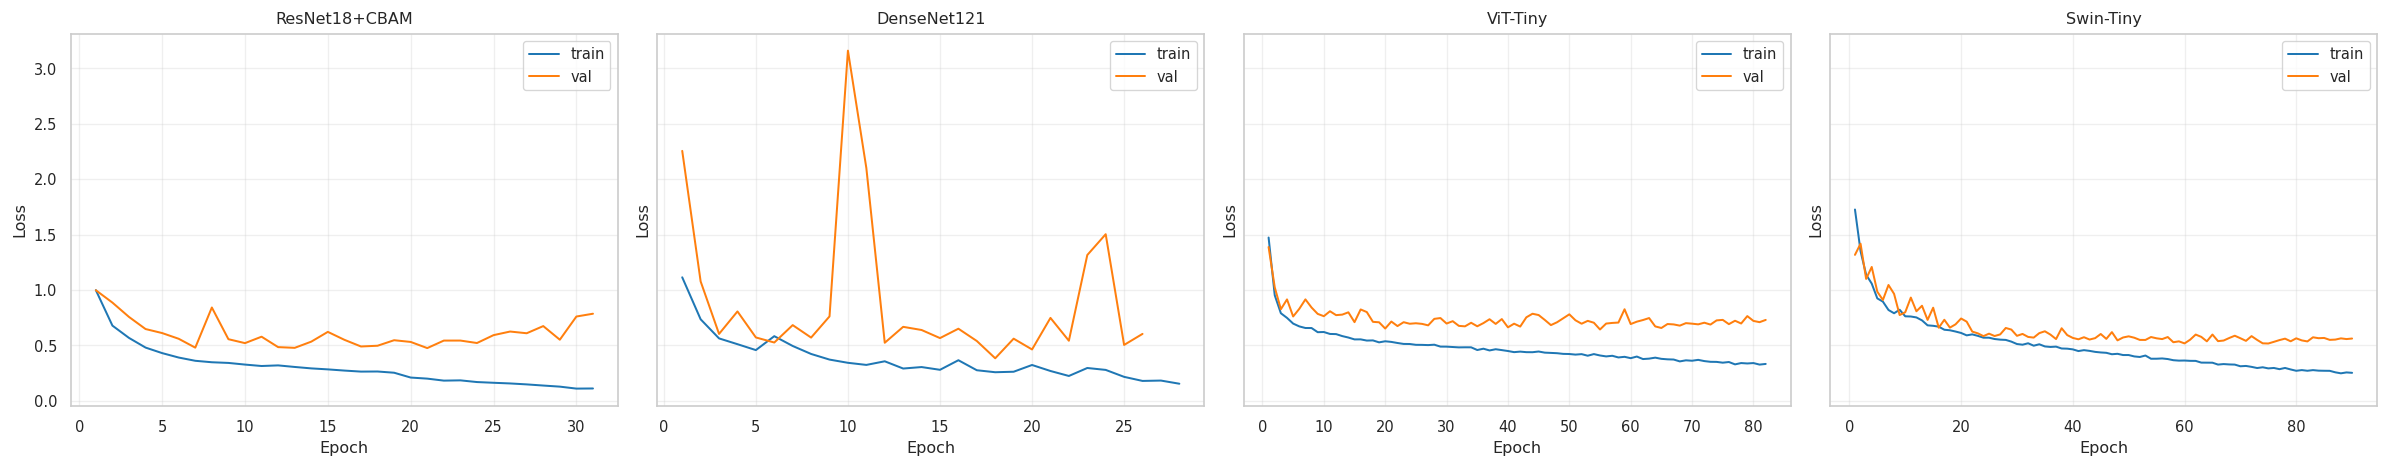
\includegraphics[width=0.70\linewidth]{fig_09.png}
\caption{\textbf{补充图 S1.} 训练与验证损失曲线（seed 42）}
\end{figure}

\phantomsection
\subsection*{S4. 完整超参数表}
\addcontentsline{toc}{subsection}{S4. 完整超参数表}

\begin{table}[htbp]
\centering
\small
\caption{\textbf{补充表 S1a.} WM-811K 各家族的训练超参数}
\resizebox{\linewidth}{!}{%
\begin{tabular}{llrrrrlrllrlr}
\toprule
家族 & 优化器 & 学习率 & 权重衰减 & 批大小 & 最大轮数 & 调度器 & 早停耐心 & 早停指标 & 损失 & 梯度裁剪 & 混合精度 & Dropout \\
\midrule
ResNet18+CBAM & adam & 0.0010 & 0.00 & 32 & 50 & reduce\_on\_plateau & 10 & val\_balanced\_acc & cross\_entropy & 1.0 & True & 0.5 \\
DenseNet121 & adam & 0.0010 & 0.00 & 32 & 50 & reduce\_on\_plateau & 10 & val\_balanced\_acc & cross\_entropy & 1.0 & True & 0.5 \\
ViT-Tiny & adamw & 0.0003 & 0.05 & 64 & 100 & cosine & 20 & val\_f1\_macro & cross\_entropy & 1.0 & True & 0.3 \\
Swin-Tiny & adamw & 0.0003 & 0.05 & 64 & 100 & cosine & 20 & val\_f1\_macro & cross\_entropy & 1.0 & True & 0.3 \\
\bottomrule
\end{tabular}
}
\end{table}

四个家族共享完全一致的数据与增强设置：64×64 图像、按批次分组 划分（70/15/15）、4 个 worker、预处理缓存、数据增强（旋转 概率 0.7、翻转概率 0.5、高斯噪声 σ=0.05 / 概率 0.3），并启用 少数类加强采样。

\begin{center}
\small \textbf{补充表 S1b.} MVTec AD 各家族的训练超参数
\end{center}

\begin{tabular}{lcccc}
\toprule
参数 & ResNet18+CBAM & DenseNet121 & ViT-Tiny (DeiT) & Swin-Tiny \\
\midrule
预训练 & ImageNet & ImageNet & ImageNet (DeiT) & ImageNet \\
优化器 & AdamW（全部相同） &  &  &  \\
学习率 & 0.0003 & 0.0003 & 0.0001 & 0.0001 \\
权重衰减 & 0.05（全部相同） &  &  &  \\
批大小 / 轮数 & 32 / 100（全部相同） &  &  &  \\
调度 & 余弦（全部相同） &  &  &  \\
早停 & 15 / val\_f1（全部相同） &  &  &  \\
损失 / AMP / Dropout & CE / ✓ / 0.5（全部相同） &  &  &  \\
图像 / 窗口 & 256² / — & 256² / — & 256² / — & 256² / 7 \\
划分 & 分层 70/15/15（全部相同） &  &  &  \\
\bottomrule
\end{tabular}


\begin{center}
\small \textbf{补充表 S2.} 可解释性评估参数（两个数据集）
\end{center}
\begin{tabular}{ll}
\toprule
参数 & 值 \\
\midrule
每次评估样本数 & WM-811K: 198/种子（9 类）；MVTec: 200 \\
Top-k 比例 & 10\% \\
Deletion/Insertion 步数 & 20 \\
扰动基线 & 零填充（背景 = 0） \\
稳定性增强次数 & 每样本 5 次 \\
稳定性变换 & 旋转 ±15°、平移 ±3 px、噪声 σ=0.02 \\
稳定性度量 & 余弦相似度（仅晶圆区域） \\
评估所用种子 & WM-811K: 7/123/456 (Swin), 42/123/456 (其他)；MVTec: 42 \\
RISE 掩码数 (N) & 4,000 \\
RISE 掩码分辨率 & 8；消融: 16, 32 (MVTec) \\
RISE 概率 (p) & 0.5 \\
IoU 阈值 & MVTec: 第 50 百分位二值化 \\
\bottomrule
\end{tabular}



\begin{table}[htbp]
\centering
\small
\caption{\textbf{补充表 S3.} 十二次运行的逐种子分类结果}
\resizebox{\linewidth}{!}{%
\begin{tabular}{lrrrrr}
\toprule
家族 & 种子 & 准确率 & 宏 F1 & 平衡准确率 & 训练轮数 \\
\midrule
ResNet18+CBAM & 42 & 0.952 & 0.843 & 0.901 & 31 \\
ResNet18+CBAM & 123 & 0.960 & 0.850 & 0.902 & 35 \\
ResNet18+CBAM & 456 & 0.959 & 0.855 & 0.899 & 36 \\
DenseNet121 & 42 & 0.959 & 0.844 & 0.912 & 28 \\
DenseNet121 & 123 & 0.960 & 0.846 & 0.897 & 36 \\
DenseNet121 & 456 & 0.967 & 0.868 & 0.895 & 35 \\
ViT-Tiny & 42 & 0.920 & 0.744 & 0.819 & 82 \\
ViT-Tiny & 123 & 0.927 & 0.739 & 0.792 & 67 \\
ViT-Tiny & 456 & 0.938 & 0.758 & 0.786 & 94 \\
Swin-Tiny & 7 & 0.955 & 0.791 & 0.809 & 90 \\
Swin-Tiny & 123 & 0.953 & 0.787 & 0.814 & 78 \\
Swin-Tiny & 456 & 0.951 & 0.797 & 0.842 & 97 \\
\bottomrule
\end{tabular}
}
\end{table}

\phantomsection
\subsection*{S5. 原始定性热图（无晶圆叠加）}
\addcontentsline{toc}{subsection}{S5. 原始定性热图（无晶圆叠加）}

正文图 5 出于可读性考虑将各热图半透明叠加在输入晶圆上。这种 合成视图可能将热图本身的行为与晶圆背景视觉上混淆。补充图 S2 使用相同样本，但去除晶圆背景并让每张热图按自身动态范围归一化。 原始视图清晰地表明：(i) ResNet18+CBAM 的 Grad-CAM 在本质上 与输入无关——九个类别上都呈现近乎相同的左上角色块；(ii) DenseNet121 的 Grad-CAM 同样被象限锁定，象限随类别变化，但 在象限内部没有形状感知；(iii) ViT-Tiny 的 Attention Rollout 确实 随输入自适应，与缺陷的空间对应在 Center 和 Loc（热点落在缺陷簇上） 以及 Edge-Ring（热点沿环形圆周分布）上最为明显；在 Donut、 Edge-Loc 与 Near-Full 上较弱。对于 None，热图缺乏连贯的缺陷形状结构（符合预期， 因为不存在缺陷信号）；对于 Random，激活模式可与 None 区分但未 跟踪弥散的缺陷像素；对于 Scratch，热点部分沿弧形轨迹分布—— 这与补充表 S4 报告的 Spearman 秩相关一致。


\begin{figure}[htbp]
\centering
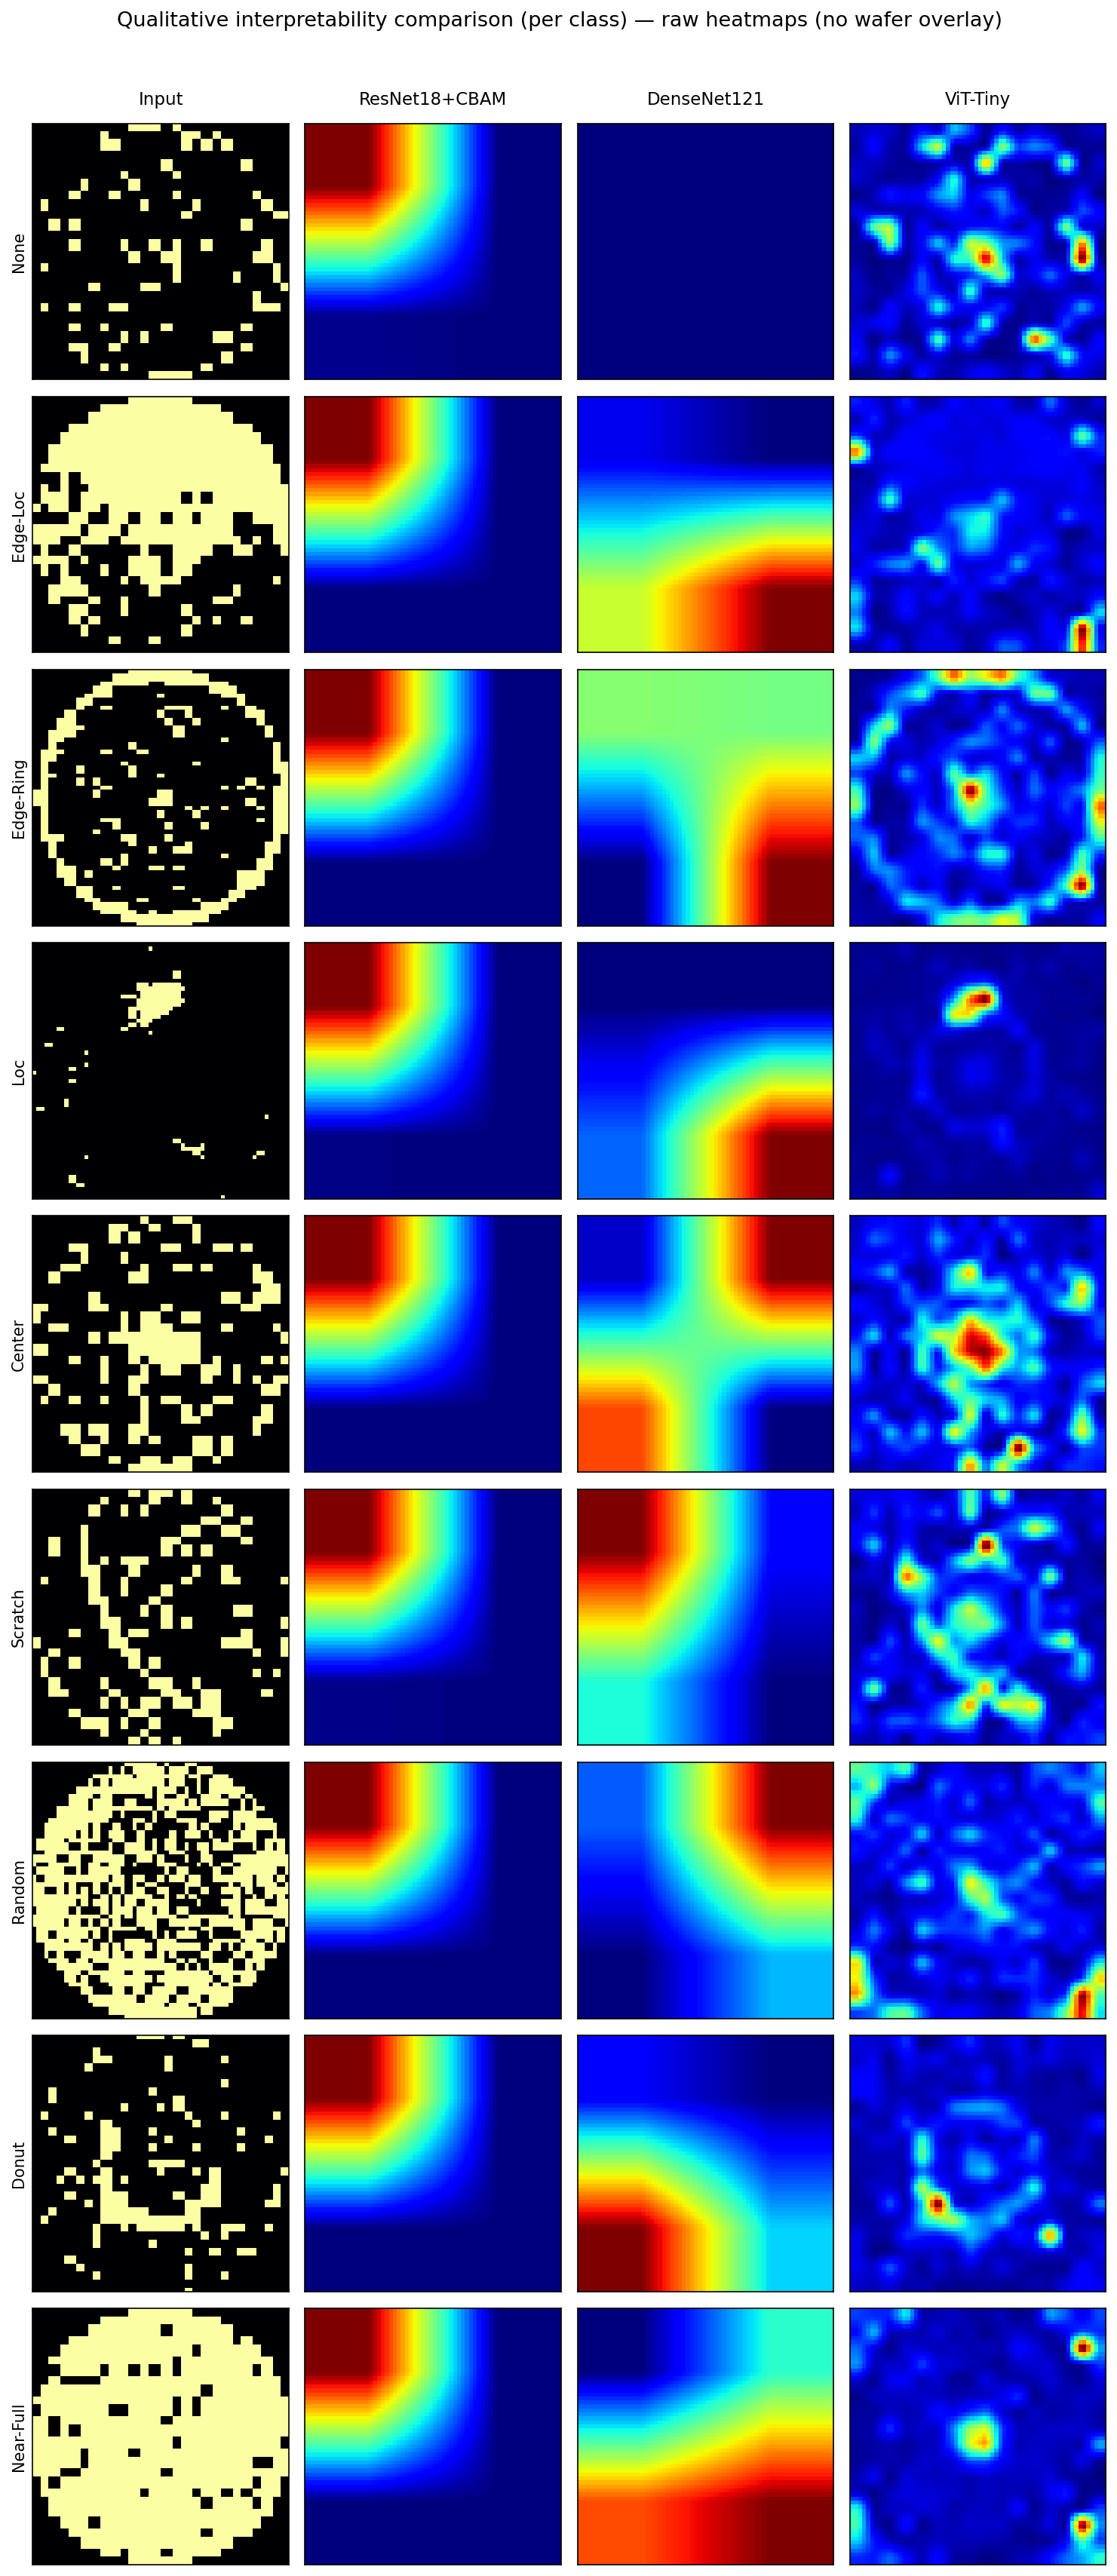
\includegraphics[width=0.60\linewidth]{fig_10.png}
\caption{\textbf{补充图 S2.} 原始定性热图（无晶圆叠加）。样本与图 5 相同；每张热图按自身 min–max 范围归一化，以便公平的视觉比较}
\end{figure}

\clearpage
\phantomsection
\subsection*{S6. 与缺陷分布的空间对齐}
\addcontentsline{toc}{subsection}{S6. 与缺陷分布的空间对齐}

为定量评估各方法的热图与晶圆缺陷像素分布的空间对齐程度，我们 计算每个样本的热图与二值缺陷掩码之间的 Spearman 秩相关，所有 594 个评估样本（每家族）的均值见补充表 S4。该相关性并不作为因果 忠实度指标使用；它仅衡量热图与标注失败芯粒像素之间的空间对齐 程度。接近零的相关系数表明热图与缺陷分布无空间对齐；较高的正 相关表明热图将强度集中在缺陷像素上。


\begin{table}[htbp]
\centering
\small
\caption{\textbf{补充表 S4.} 热图强度与晶圆缺陷像素分布之间的 Spearman 秩相关（每家族 n=594 样本）。数值接近零表示无空间对齐}
\begin{tabular}{lrr}
\toprule
家族 & 缺陷相关性（均值） & 缺陷相关性（标准差） \\
\midrule
ResNet18+CBAM & 0.037 & 0.105 \\
DenseNet121 & 0.015 & 0.126 \\
ViT-Tiny & 0.318 & 0.209 \\
Swin-Tiny & 0.042 & 0.105 \\
\bottomrule
\end{tabular}
\end{table}



\phantomsection
\subsection*{S7. 逐种子 Deletion AUC}
\addcontentsline{toc}{subsection}{S7. 逐种子 Deletion AUC}

为支持 §5.1 中关于“忠实度排序在不同随机种子下稳定”的论述， 下表报告每个种子上各家族的 Deletion AUC 均值。每个单元格 在 200 个均衡分层采样样本上取均值。


\begin{table}[htbp]
\centering
\small
\caption{\textbf{补充表 S5.} 逐种子 Deletion AUC 均值（每种子 200 个均衡分层样本）}
\begin{tabular}{lllrr}
\toprule
家族 & seed 7 & seed 42 & seed 123 & seed 456 \\
\midrule
DenseNet121 & NaN & 0.544 & 0.514 & 0.519 \\
ResNet18+CBAM & NaN & 0.486 & 0.512 & 0.485 \\
Swin-Tiny & 0.44 & NaN & 0.413 & 0.444 \\
ViT-Tiny & NaN & 0.221 & 0.223 & 0.188 \\
\bottomrule
\end{tabular}
\end{table}



\phantomsection
\subsection*{S8. 消融：随机像素基线}
\addcontentsline{toc}{subsection}{S8. 消融：随机像素基线}

为校准 Deletion/Insertion 指标，我们将各方法的热图排序替换为 均匀随机像素排列，并在 seed-42 模型上重新运行相同扰动协议 （198 个分层样本）。

\begin{table}[htbp]
\centering
\small
\caption{\textbf{补充表 S6.} 基于热图 vs 随机像素的 Deletion/Insertion AUC，WM-811K（seed 42）}
\begin{tabular}{lrrrr}
\toprule
family & Del（热图） & Ins（热图） & Del（随机） & Ins（随机） \\
\midrule
densenet121 & 0.544 & 0.501 & 0.508 & 0.494 \\
resnet18\_cbam & 0.486 & 0.531 & 0.498 & 0.492 \\
swin\_tiny & 0.440 & 0.448 & 0.475 & 0.453 \\
vit\_tiny & 0.221 & 0.689 & 0.480 & 0.480 \\
\bottomrule
\end{tabular}
\end{table}

CNN Grad-CAM 排序不优于随机排列（ResNet Del 0.486 vs 随机 0.498； DenseNet Del 0.544 vs 随机 0.508——均处于或高于随机水平），表明 高亮像素携带的预测相关信号不超过机会水平。ViT-Tiny Rollout（Del 0.221） 明显优于随机基线（0.480），提供了更强的扰动式忠实度证据。

在 MVTec AD 上，RISE Deletion AUC 仍然较高（各家族和掩码分辨率 下为 0.66–0.94），与该扰动协议在 MVTec 数据集（§4.7）上有限的 忠实度一致。

\clearpage
\phantomsection
\subsection*{S9. 消融：ViT 上的 Grad-CAM（非原生对照）}
\addcontentsline{toc}{subsection}{S9. 消融：ViT 上的 Grad-CAM（非原生对照）}

为将架构效应与解释器效应解耦，我们对 Attention Rollout 所解释的 同一 ViT-Tiny 模型施加 Grad-CAM（目标层为最后一个 Transformer 编码器层）。这是一个刻意的非原生对照：Grad-CAM 为卷积特征图 设计，而非 Transformer token 序列。

\begin{table}[htbp]
\centering
\small
\caption{\textbf{补充表 S7.} ViT-Tiny：原生（Rollout）vs 非原生（Grad-CAM）解释器}
\begin{tabular}{lrr}
\toprule
方法 & Deletion AUC ↓ & Insertion AUC ↑ \\
\midrule
Attention Rollout（原生） & 0.221 & 0.689 \\
Grad-CAM（非原生） & 0.492 & 0.488 \\
\bottomrule
\end{tabular}
\end{table}

ViT 上的 Grad-CAM 产生与随机无异的忠实度（Del 0.492 vs 随机 0.480），而同一模型上的 Rollout 达到 Del 0.221。这表明忠实度 优势归因于原生读出解释器，而非 ViT 架构或其 patch 级空间粒度。

\phantomsection
\subsection*{S10. 消融：最后一层 CLS 注意力（Rollout 深度对照）}
\addcontentsline{toc}{subsection}{S10. 消融：最后一层 CLS 注意力（Rollout 深度对照）}

为解耦读出直接性与 Rollout 深度，我们评估 ViT-Tiny 最后一层 CLS-to-patch 注意力：最后一个 Transformer 块的注意力权重从 [CLS] 查询到所有 patch token，在头之间平均。这保持读出来源不变 （原生注意力矩阵），同时移除完整 Attention Rollout 所用的 12 层 递归传播。

\begin{tabular}{llll}
\toprule
方法 & 读出 & 深度 & Del AUC ↓ \\
\midrule
完整 Rollout & 原生注意力 & 12 层递归 & 0.211 \\
最后一层 CLS 注意力 & 原生注意力 & 单层 & 0.367 \\
ViT Grad-CAM (S9) & 非原生（梯度） & 单层 & 0.492 \\
CNN Grad-CAM & 非原生（梯度） & 单层 & 0.495–0.525 \\
\bottomrule
\end{tabular}


\textbf{表 S10.} ViT 忠实度优势的 2×2 分解。 最后一层 CLS 注意力（3 种子均值，每种子 n=198）。 种子：Del 0.340 / 0.401 / 0.359（均值 0.367 ± 0.031）。

实现说明：最后一层注意力取最后一个块的原始 [CLS]-to-patch 注意力 行（头间平均），不使用完整 Rollout 中的残差校正（½A + ½I）。

完整 Rollout 与 CNN Grad-CAM 的总差距约为 0.30。最后一层注意力 落在 0.367，将差距分解为：

\begin{itemize}
\item \textbf{读出直接性}（最后一层注意力 vs ViT Grad-CAM）： 0.492 − 0.367 = 0.125（≈42\%）
\item \textbf{Rollout 深度}（完整 Rollout vs 最后一层注意力）： 0.367 − 0.211 = 0.156（≈52\%）
\end{itemize}

两个结构代理均携带独立信号。读出直接性单独已优于同一模型上的 非原生 Grad-CAM 对照，而多层 Rollout 贡献了可比的额外改善 （≈0.16）。该分解是路径依赖的（残余 ≈6\% 反映非可加性）。

\textbf{MVTec AD 对比（seed 42，n=200 缺陷样本）：}

\begin{tabular}{ll}
\toprule
方法 & Del AUC ↓ \\
\midrule
RISE & 0.656 \\
完整 Rollout & 0.770 \\
最后一层 CLS 注意力 & 0.857 \\
\bottomrule
\end{tabular}


在 MVTec 上模式反转：最后一层注意力最差，完整 Rollout 部分改善， 但 RISE 超越两种原生方法。这表明 MVTec 边界条件并非简单的 Rollout 深度问题；预训练注意力通路似乎仅部分对齐于微调后的 决策边界。

\phantomsection
\subsection*{S11. 消融：共同正确子集}
\addcontentsline{toc}{subsection}{S11. 消融：共同正确子集}

为排除“较弱分类器产生人为忠实解释”的替代解释（因为更简单的 决策边界依赖更少像素），我们将评估限制在主种子中四个家族 均正确分类的 140 个样本（共 198 个）上。

\begin{table}[htbp]
\centering
\small
\caption{\textbf{补充表 S11.} 仅对共同正确样本的忠实度}
\begin{tabular}{lrrrr}
\toprule
family & Del AUC (mean) & Del AUC (std) & Ins AUC (mean) & Ins AUC (std) \\
\midrule
densenet121 & 0.554 & 0.273 & 0.518 & 0.264 \\
resnet18\_cbam & 0.499 & 0.260 & 0.543 & 0.220 \\
swin\_tiny & 0.452 & 0.231 & 0.456 & 0.213 \\
vit\_tiny & 0.216 & 0.213 & 0.711 & 0.316 \\
\bottomrule
\end{tabular}
\end{table}

家族排序完全保持甚至略有放大（ViT Del 0.216 vs CNN 0.50–0.55）。 忠实度差距不能归因于分类准确率差异。

\phantomsection
\subsection*{S12. 消融：top-k 敏感性}
\addcontentsline{toc}{subsection}{S12. 消融：top-k 敏感性}

为验证家族排序并非 10 \% 扰动阈值的伪影，我们测量仅移除热图 排序前 5 \%、10 \% 或 20 \% 像素后的置信度下降。

\begin{table}[htbp]
\centering
\small
\caption{\textbf{补充表 S12.} 移除 top-k\% 像素后的平均置信度下降（Δp）}
\begin{tabular}{lrrr}
\toprule
family & top-5\% & top-10\% & top-20\% \\
\midrule
densenet121 & 0.106 & 0.142 & 0.238 \\
resnet18\_cbam & 0.029 & 0.046 & 0.136 \\
swin\_tiny & 0.034 & 0.086 & 0.210 \\
vit\_tiny & 0.362 & 0.492 & 0.589 \\
\bottomrule
\end{tabular}
\end{table}

ViT-Tiny Rollout 的顶部像素在每种粒度下都对预测至关重要 （Δp = 0.36 @ 5 \%、0.49 @ 10 \%、0.59 @ 20 \%），而 CNN Grad-CAM 像素产生的置信度变化极小（ResNet Δp = 0.03–0.14）。家族排序 在所有三个阈值下均稳定，表明结果对扰动粒度不敏感。


\phantomsection
\subsection*{S13. Swin-Tiny 补充细节}
\addcontentsline{toc}{subsection}{S13. Swin-Tiny 补充细节}

\begin{center}
\small \textbf{补充表 S13.} Swin-Tiny 配置与结果概览
\end{center}

\begin{tabular}{lcc}
\toprule
属性 & WM-811K（从头训练） & MVTec AD（预训练） \\
\midrule
参数量 & 27,504,723 & 27,520,892 \\
输入尺寸 & 64×64，单通道 & 256×256，3通道 RGB \\
窗口大小 & 4 & 7 \\
预训练 & 否 & ImageNet \\
种子 & 7, 123, 456 & 42 \\
训练轮数（均值） & 88 & 57 \\
平衡准确率 & 82.2 ± 1.5\% & 93.7\% \\
F1 Macro & 0.792 ± 0.004 & 0.947 \\
Grad-CAM 目标层 & \texttt{layers[-1]} & \texttt{layers[-1]} \\
原生 Del AUC & 0.432 ± 0.017 & 0.509 \\
原生 Ins AUC & 0.480 ± 0.028 & 0.909 \\
稳定性 & 0.893 ± 0.006 & — \\
RISE Del AUC & 0.096 & 0.709 \\
\bottomrule
\end{tabular}


\textbf{架构。} Swin-Tiny [23] 使用移位窗口自注意力，包含 4 个层级 阶段。在 WM-811K（64×64，单通道）上窗口大小设为 4；在 MVTec AD （256×256，3 通道 RGB）上使用默认窗口大小 7。模型参数量为 27.5M。

\textbf{种子选择（WM-811K）。} 种子 42 产生退化初始化，未能收敛 （BAcc 23.4\%，第 21 轮早停）。替换为种子 7，得到 BAcc 80.9\%。 种子 123 和 456 正常收敛（分别为 81.4\% 和 84.2\%）。

\textbf{Grad-CAM 目标层。} 使用最终 Transformer 阶段 （\texttt{model.backbone.layers[-1]}）作为 Grad-CAM 目标层。

\phantomsection
\subsection*{S14. 代码与数据可用性}
\addcontentsline{toc}{subsection}{S14. 代码与数据可用性}

完整的源代码、配置文件以及 WM-811K 和 MVTec AD 两个数据集的 评估脚本均公开可用：

\textbf{代码仓库：} https://github.com/JasperJia33/native-readout-xai

WM-811K 数据集 [18] 公开可用。MVTec AD [19] 可从 MVTec 网站以学术许可获取。


\end{document}